\documentclass[preprint,12pt,authoryear]{elsarticle}

\usepackage{graphicx}% Include figure files
\usepackage{latexsym}
\usepackage{etoolbox}
\usepackage{pstricks, pst-node, pst-text, pst-3d}
\usepackage{amssymb, amsmath, amscd, amsbsy}
\usepackage{mathptmx, mathrsfs, mathtools, mathdots}
\usepackage{verbatim}
\usepackage{hyperref}
\usepackage{placeins}
\usepackage{multirow}
\usepackage{dcolumn}% Align table columns on decimal point 
\usepackage{pifont}
\usepackage{colortbl}
\usepackage{xcolor}

\definecolor{Myred}{rgb}{1,0.5,0.5}
\definecolor{Mygreen}{RGB}{144,238,144}
\definecolor{MyYellow}{HTML}{FFFFE0}
\definecolor{MyBlue}{RGB}{173,216,230}

\usepackage{lipsum}
\usepackage{upgreek} % Greek letter
\usepackage{cancel} % arrow
\usepackage{array}
\usepackage{color}
\usepackage{float}
\usepackage{tikz}
\usepackage{bm}% bold math

\usepackage{lineno}

\usepackage{natbib}
\bibliographystyle{aipnum4-1}
\setcitestyle{numbers,square}

\date{April 14, 2025}

\begin{document}

\begin{frontmatter}
%
\title{Study of the electron to ion root transition using Langmuir probes}
\date{April 14, 2025}
%\author{Arnold A. Alvarez$^{1}$, Eduardo L. Brugnago$^{1}$ and I. L. Caldas$^{1}$}
%\address{$^1$Instituto de F\'isica, Universidade de S\~ao Paulo, S\~ao Paulo, SP, Brasil.}
\author{Arnold A. Alvarez}%$^{1}$,  B.Ph. van Milligen$^{2}$, and I. L. Caldas$^{1}$}
%\address{Instituto de F\'isica, Universidade de S\~ao Paulo, S\~ao Paulo, SP, Brasil.}
%\address{National Fusion Laboratory, CIEMAT, Madrid, Spain}

%        
%\cortext[cor]{Corresponding author: arnold@if.usp.br}
%
\date{\today}
%
\begin{abstract}
    bla bla bla 
\end{abstract}

\begin{keyword}
    bla bla bla
\end{keyword}
%
\end{frontmatter}

\section{Introduction}


{\em This section needs to discuss (1) the issue to investigate (impact of ECRH heating power on turbulence), (2) antecedents and previous studies both at TJ-II and elsewhere, (3) motivation and goals of this work.}

The electron to ion (e-i) root transition is an important phenomenon in stellarators, associated with the sign reversal of the radial electric field in the plasma edge.
It is a confinement transition that involves the spontaneous generation of a transport barrier in the edge plasma region, and therefore is in the same category of transitions as the important L--H (low to high confinement) transition and the formation of Internal Transport Barriers (ITBs) \cite{Ida:2020}.

In the TJ-II stellarator, the electron to ion root confinement transition has been studied extensively \cite{Hidalgo:2006b}.
The transition was generally found to occur when the line averaged electron density, $n_e$ exceeds a threshold value of $n_{e,c} \simeq 0.6 \cdot 10^{19}$ m$^{-3}$ \cite{Pedrosa:2005,Pedrosa:2005c}.
The transition is characterized by an increase of fluctuation levels and the occurrence of long range correlations, characteristic of zonal flows \cite{Pedrosa:2008}.

The control parameter of this transition is however unlikely to be the line average density directly;
rather, it seems to be controlled by the value of the radial electric field in the plasma edge region.

The evolution of the potential profile at TJ-II has been documented in some detail \cite{Melnikov:2011}.
The potential drops gradually as the electron density increases, and near the critical density $n_{e,c}$ it changes sign.
As a consequence, the edge radial electric field indeed tends to change sign when $n_e$ crosses the critical value.

There is however a second parameter that modifies the plasma potential: the Electron Cyclotron Resonance Heating (ECRH) power.
In \cite{Melnikov:2011} it was also reported that the potential increases with higher ECRH power.
Consequently, as ECRH power is switched off, the plasma potential becomes more negative and often, if the electron density is slightly below the critical density, this triggers an e-i confinement transition.
This effect is regularly observed in TJ-II discharges.

Here, we perform a detailed study of the response of the plasma near the e-i root transition to the modulation of ECRH power.
This study complements earlier work at TJ-II in which global transport was studied with ECRH power modulation \cite{S_Eguilior_2003}, or transport was studied as a function of ECRH power \cite{Milligen:2018b}, or modulated electrode biasing was applied, affecting the edge radial electric field and transport \cite{Grenfell:2019}.

The novelty of this work lies in the analysis of the response of turbulence to ECRH modulation.
For this purpose, we will make use of an array of quantifiers and will attempt to show that the e-i transition can be qualified as a `phase transition', characterized by a change of system order.

{\em Previous relevant work on other devices: ...}

\section{Experimental Set-up}

\section{Methods}

\subsection{TJ-II stellarator}

Describe TJ-II: parameters, heating, fueling, etc. Also, we need to summarize what we know about the electron-to-ion root transition at TJ-II. 
It occurs systematically at a critical density $n_{e,c} \simeq 0.6 \cdot 10^{19}$ m$^{-3}$
\cite{Hidalgo:2006b} \cite{Pedrosa:2008}.
As the density increases, the global potential profile goes from positive to negative, the inversion starting from the plasma edge and moving inward. This leads to the formation of a shear layer at the plasma edge and one can detect long-range correlations (between the 2 Langmuir probes), associated with zonal flows, if they are placed at the right radial position.

\subsection{Diagnostics}

Describe diagnostics (only if used): ECE, Langmuir probes, HIBP, Thomson Scattering, He-Beam, magnetics (if applicable; use previous articles and the \href{https://wiki.fusion.ciemat.es/wiki/TJ-II}{Fusionwiki} for inspiration and references).

The 2-D probe has a specific configuration that allows computing some interesting quantities, including $T_e$.
An estimate of the turbulent radial particle flux is possible $\Gamma \propto \tilde I_{sat} \tilde E_\theta$.
The probe also allows estimating the Reynolds Stress term $R = \langle \tilde E_r \tilde E_\theta \rangle$, important for the formation of transport barriers (it describes the energy transfer from fluctuations to mean flow).
This section should describe in detail how to do all that.

\subsection{Analysis Methods}

The analysis of single time traces may include the mean, RMS, Skewness, Kurtosis (of $V_f, I_{sat}, \dots$), spectra, etc. From the multipin probes, we may obtain the radial electric field $E_r$, the poloidal velocity $v_{corr} \simeq v_\theta$ \cite{Milligen:2023b}, the radial fluctuating particle flux $\Gamma \propto \tilde I_{sat} \tilde E_\theta$, the Reynolds Stress $R = \langle \tilde E_r E_\theta \rangle$, the intermittence \cite{Carreras:2020}. Profiles of these quantities. 

Radial correlations of various quantities (such as the floating potential) may provide evidence of radial propagation and its velocity. One may try radial correlation of HIBP and Langmuir potential. One may also look at Transfer Entropy.

Toroidal correlations between Langmuir probe $V_f$ measurements indicate the existence of zonal flows \cite{Pedrosa:2008}, \cite{Milligen:2015}: variation with $P_{ECRH}$ and radius.

Once we get an idea of how things change with $P_{ECRH}$ 'high' and 'low' and $n_e$ (in a few selected shots), we might also want to see {\em how fast} the plasma responds to the change in $P_{ECRH}$, and/or how these changes propagate. Do mean profiles respond before the turbulence changes? Or (more likely), does the turbulence change before the profiles do? 

\section{Experimental results}

\subsection{Experiments}


\begin{figure}[!ht]
   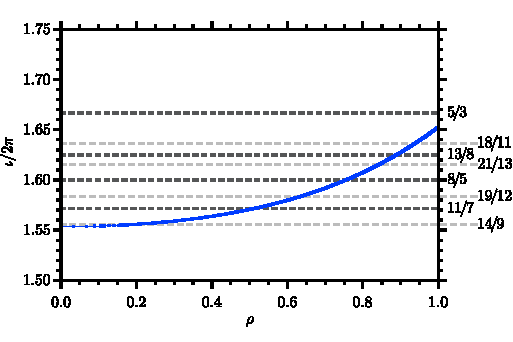
\includegraphics[width=264 pt]{Images/Figure1.pdf}
   \caption{Profile of $\iota/2\pi$ for the magnetic configuration 100\_44\_64, and some rotational values are indicated by horizontal dashed lines.}
   \label{Fig:Figure1}
\end{figure}

Describe experiments (day, heating power $P_{ECRH}$ +  modulation, density variation). Magnetic configuration (see Fig. \ref{Fig:Figure1}).
Clarify that high $n_e$ means low $T_e$, hence high collisionality. This will affect transport.

Distinguish between shots with different line average densities: below, at, and above the `critical density' of $n_{e,c} \simeq 0.6 \cdot 10^{19}$ m$^{-3}$.
A few representative time traces are shown in Fig. \ref{Fig:Densities_1}.
This figure is rather interesting and key to this study: The time traces with $n_e \simeq n_{e,c}$ seem to show that it is possible to create and destroy the edge transport barrier using ECRH modulation!

\begin{figure}[!ht]
\centering
   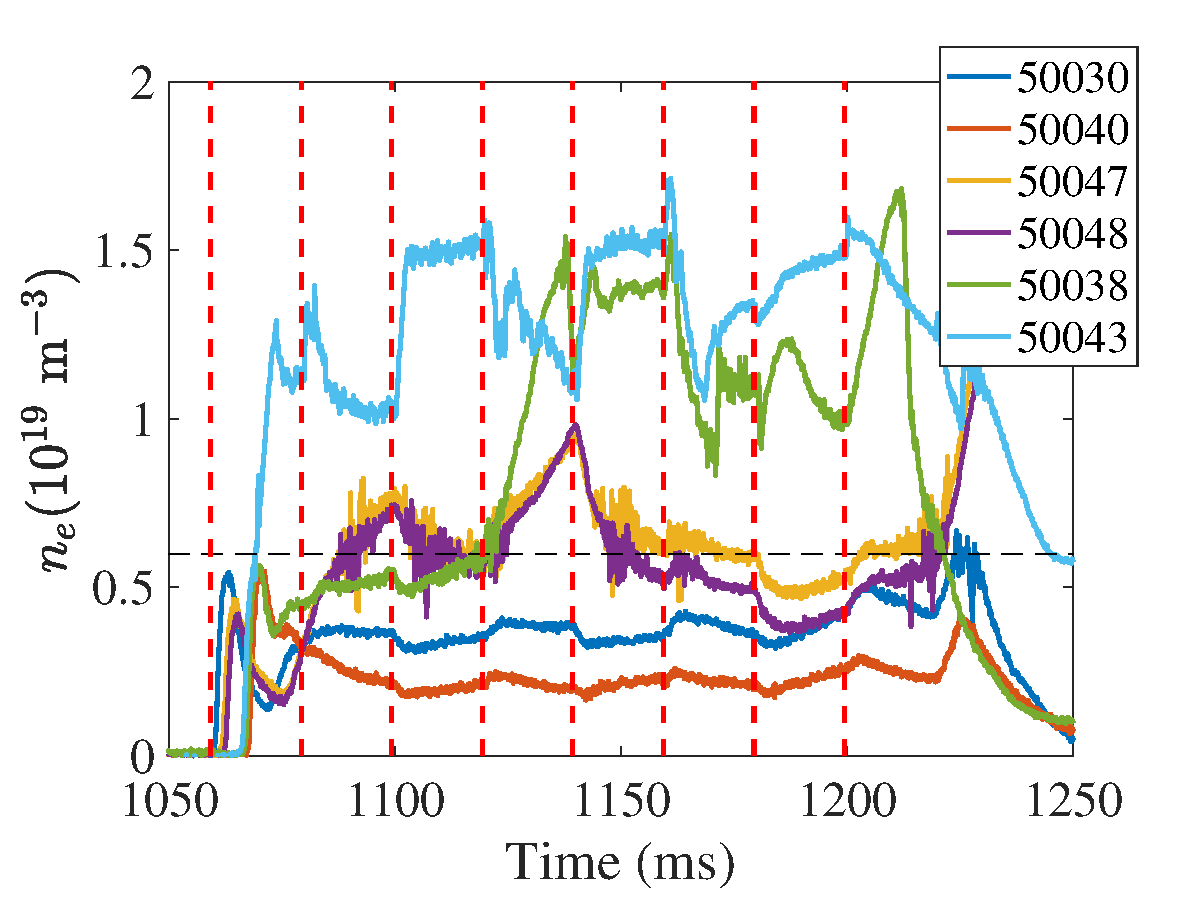
\includegraphics[width=0.75\columnwidth]{Images/Densities.eps}
   \caption{Density traces of some shots with ECRH modulation, showing the resulting modulation of $n_e$. ECRH switching times are indicated by vertical dashed lines. The critical density $n_{e,c} \simeq 0.6 \cdot 10^{19}$ m$^{-3}$ is indicated by a horizontal dashed line. Shots 50030 and 50040 have $n_e < n_{e,c}$ and the density modulated in counter-phase with $P_{ECRH}$. Shots 50047 and 50048 have $n_e \simeq n_{e,c}$ and in at least one time interval, the density increases rapidly due to improved confinement associated with an edge transport barrier. This rapid increase happens during a $P_{ECRH}$ off state; in this state, the density (gradient) rises slightly, which may trigger the barrier. Shot 50043 has $n_e > n_{e,c}$ and reversed $n_e$ modulation (50038 has at least one similar modulation period, following the establishment of the edge transport barrier, indicated by a period of rapid increase of the density).}
   \label{Fig:Densities_1}
\end{figure}

Preliminary classification of shots (to be checked/improved):
\begin{itemize}
\item $n_e < n_{e,c}$: 50019-50030, 50037, 50039-50040
\item $n_e \simeq n_{e,c}$: 50031-50036, 50041-50042, 50044-50048, 50050-50053. The confinement transition is visible as a noise on the interferometry time trace \cite{Milligen:2011}.
\item $n_e > n_{e,c}$: 50038, 50043
\end{itemize}

The GR modulation leads to a separate classification:
\begin{itemize}
\item shot $\le$ 50037: GR on axis
\item 50038 $\le$ shot $\le$ 50052: GR off axis
\item shot $\ge$ 50053: GR2 on axis
\end{itemize}

Present an inventory of these experiments, showing profiles for both heating phases (ECRH on/off), for all classes of mean $n_e$ above. Profiles may include: ECE, Thomson Scattering, HIBP, Langmuir (and maybe Helium beam). Avoid transitionary states immediately following ECRH switching times.

\subsection{Thomson Scattering profiles}

Document the Thomson Scattering profiles, and see to which modulation phase they correspond (see script plot\_Thomson.m). For example, Fig. \ref{Fig:Thomson} shows mean Thomson Scattering $T_e$ profiles during the ECRH on and off phases, for shots with on-axis modulation.

\begin{figure}[!ht]
\centering
   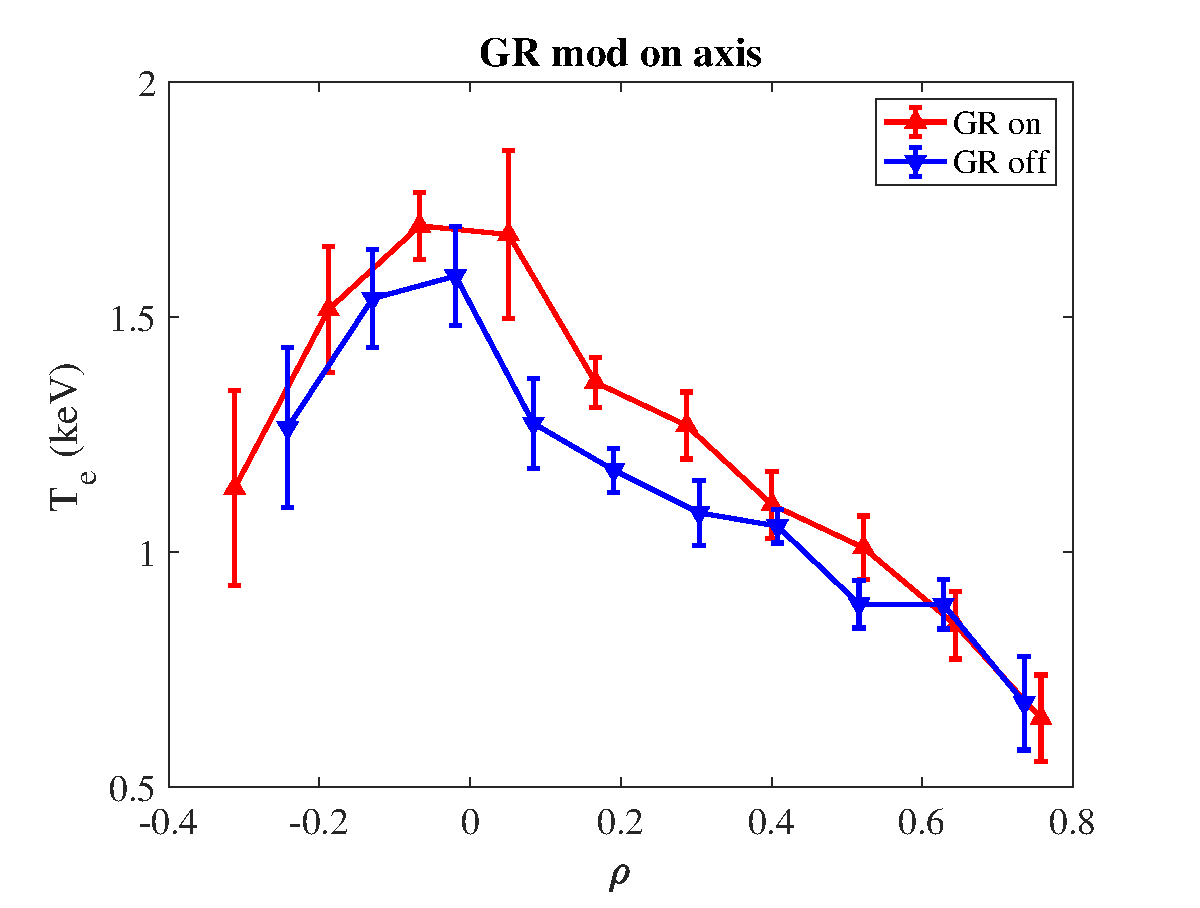
\includegraphics[width=0.5\columnwidth]{Images/Thomson.eps}
   \caption{Mean Thomson Scattering profiles for ECRH on / off (shots [50019:50034,50036]).Shots with both low and medium density (better separate them?).}
   \label{Fig:Thomson}
\end{figure}

\subsection{Heavy Ion Beam Probe profiles}

Document the HIBP profiles (from scanned shots). We have the following data:

\begin{center}
\begin{table}[!ht]
\scriptsize
    \begin{tabular}{|| c || c | c | c | c | c | c | c | c ||} 
        \hline
        Shot & On/Off axis & GR1 & GR2 & D (p. depth) &  B (p. depth) & NBI & HIBP1 & HIBP2  \\ [0.5ex] 
        \hline\hline
        50019 & On\cellcolor{MyYellow}& Modulated\cellcolor{Mygreen} & Non-Modulated\cellcolor{Myred} & 600 & 290 & Off\cellcolor{Myred} & Scanned\cellcolor{Mygreen} & scanned\cellcolor{Mygreen}\\
        \hline
        50020 & On\cellcolor{MyYellow}& Modulated\cellcolor{Mygreen} & Non-Modulated\cellcolor{Myred} & 600 & 290 & Off\cellcolor{Myred} & Scanned\cellcolor{Mygreen} & scanned\cellcolor{Mygreen}\\
        \hline
        50021 & On\cellcolor{MyYellow}& Modulated\cellcolor{Mygreen} & Non-Modulated\cellcolor{Myred} & 620 & 285 & Off\cellcolor{Myred} & Fixed\cellcolor{Myred} & Fixed\cellcolor{Myred}\\
        \hline
        50022 & On\cellcolor{MyYellow}& Modulated\cellcolor{Mygreen} & Non-Modulated\cellcolor{Myred} & 640 & 282 & Off\cellcolor{Myred} & Fixed\cellcolor{Myred} & Fixed\cellcolor{Myred}\\
        \hline
        50023 & On\cellcolor{MyYellow}& Modulated\cellcolor{Mygreen} & Non-Modulated\cellcolor{Myred} & 630 & 282 & Off\cellcolor{Myred} & Fixed\cellcolor{Myred} & Fixed\cellcolor{Myred}\\
        \hline
        50024 & On\cellcolor{MyYellow}& Modulated\cellcolor{Mygreen} & Non-Modulated\cellcolor{Myred} & 650 & 282 & Off\cellcolor{Myred} & Fixed\cellcolor{Myred} & Fixed\cellcolor{Myred}\\
        \hline
        50025 & On\cellcolor{MyYellow}& Modulated\cellcolor{Mygreen} & Non-Modulated\cellcolor{Myred} & 652 & 282 & Off\cellcolor{Myred} & Fixed\cellcolor{Myred} & Fixed\cellcolor{Myred}\\
        \hline
        50026 & On\cellcolor{MyYellow}& Modulated\cellcolor{Mygreen} & Non-Modulated\cellcolor{Myred} & 655 & 278 & Off\cellcolor{Myred} & Fixed\cellcolor{Myred} & Fixed\cellcolor{Myred}\\
        \hline
        50027 & On\cellcolor{MyYellow}& Modulated\cellcolor{Mygreen} & Non-Modulated\cellcolor{Myred} & 660 & 274 & Off\cellcolor{Myred} & Fixed\cellcolor{Myred} & Fixed\cellcolor{Myred}\\
        \hline
        50028 & On\cellcolor{MyYellow}& Modulated\cellcolor{Mygreen} & Non-Modulated\cellcolor{Myred} & 670 & 272 & Off\cellcolor{Myred} & Fixed\cellcolor{Myred} & Fixed\cellcolor{Myred}\\
        \hline
        50029 & On\cellcolor{MyYellow}& Modulated\cellcolor{Mygreen} & Non-Modulated\cellcolor{Myred} & 680 & 272 & Off\cellcolor{Myred} & Fixed\cellcolor{Myred} & Fixed\cellcolor{Myred}\\
        \hline
        50030 & On\cellcolor{MyYellow}& Modulated\cellcolor{Mygreen} & Non-Modulated\cellcolor{Myred} & 685 & 270 & Off\cellcolor{Myred} & Fixed\cellcolor{Myred} & Fixed\cellcolor{Myred}\\
        \hline
        50031 & On\cellcolor{MyYellow}& Modulated\cellcolor{Mygreen} & Non-Modulated\cellcolor{Myred} & 690 & 268 & Off\cellcolor{Myred} & Fixed\cellcolor{Myred} & Fixed\cellcolor{Myred}\\
        \hline
        50032 & On\cellcolor{MyYellow}& Modulated\cellcolor{Mygreen} & Non-Modulated\cellcolor{Myred} & 690 & 266 & Off\cellcolor{Myred} & Fixed\cellcolor{Myred} & Fixed\cellcolor{Myred}\\
        \hline
        50033 & On\cellcolor{MyYellow}& Modulated\cellcolor{Mygreen} & Non-Modulated\cellcolor{Myred} & 690 & 264 & Off\cellcolor{Myred} & Fixed\cellcolor{Myred} & Fixed\cellcolor{Myred}\\
        \hline
        50034 & On\cellcolor{MyYellow}& Modulated\cellcolor{Mygreen} & Non-Modulated\cellcolor{Myred} & 690 & 262 & Off\cellcolor{Myred} & Fixed\cellcolor{Myred} & Fixed\cellcolor{Myred}\\
        \hline
        50035 & On\cellcolor{MyYellow}& Modulated\cellcolor{Mygreen} & Non-Modulated\cellcolor{Myred} & 690 & 260 & Off\cellcolor{Myred} & Fixed\cellcolor{Myred} & Fixed\cellcolor{Myred}\\
        \hline
        50036 & On\cellcolor{MyYellow}& Modulated\cellcolor{Mygreen} & Non-Modulated\cellcolor{Myred} & 690 & 260 & Off\cellcolor{Myred} & Fixed\cellcolor{Myred} & Fixed\cellcolor{Myred}\\
        \hline
        50037 & On\cellcolor{MyYellow}& Modulated\cellcolor{Mygreen} & Non-Modulated\cellcolor{Myred} & 690 & 260 & Off\cellcolor{Myred} & Fixed\cellcolor{Myred} & Fixed\cellcolor{Myred}\\
        \hline
        50038 & Off\cellcolor{MyBlue} & Modulated\cellcolor{Mygreen} & Non-Modulated\cellcolor{Myred} & 690 & 260 & Off\cellcolor{Myred} &  & \\
        \hline
        50039 & Off\cellcolor{MyBlue} & Modulated\cellcolor{Mygreen} & Non-Modulated\cellcolor{Myred} & 685 & 264 & Off\cellcolor{Myred} &  & \\
        \hline
        50040 & Off\cellcolor{MyBlue} & Modulated\cellcolor{Mygreen} & Non-Modulated\cellcolor{Myred} & 660 & 274 & Off\cellcolor{Myred} &  & \\
        \hline
        50041 & Off\cellcolor{MyBlue} & Modulated\cellcolor{Mygreen} & Non-Modulated\cellcolor{Myred} & 630 & 282 & On\cellcolor{Mygreen} &  & \\
        \hline
        50042 & Off\cellcolor{MyBlue} & Modulated\cellcolor{Mygreen} & Non-Modulated\cellcolor{Myred} & 600 & 282 & On\cellcolor{Mygreen} &  & \\
        \hline
        50043 & Off\cellcolor{MyBlue} & Modulated\cellcolor{Mygreen} & Non-Modulated\cellcolor{Myred} & 620 & 282 & On\cellcolor{Mygreen} &  & \\
        \hline
        50044 & Off\cellcolor{MyBlue} & Modulated\cellcolor{Mygreen} & Non-Modulated\cellcolor{Myred} & 620 & 282 & On\cellcolor{Mygreen} &  & \\
        \hline
        50045 & Off\cellcolor{MyBlue} & Modulated\cellcolor{Mygreen} & Non-Modulated\cellcolor{Myred} & 640 & 282 & On\cellcolor{Mygreen} &  & \\
        \hline
        50046 & Off\cellcolor{MyBlue} & Modulated\cellcolor{Mygreen} & Non-Modulated\cellcolor{Myred} & 645 & 282 & On\cellcolor{Mygreen} &  & Fixed\cellcolor{Myred}\\
        \hline
        50047 & Off\cellcolor{MyBlue} & Modulated\cellcolor{Mygreen} & Non-Modulated\cellcolor{Myred} & 655 & 276 & On\cellcolor{Mygreen} & Scanned\cellcolor{Mygreen} & Scanned\cellcolor{Mygreen}\\
        \hline
        50048 & Off\cellcolor{MyBlue} & Modulated\cellcolor{Mygreen} & Non-Modulated\cellcolor{Myred} & 665 & 274 & On\cellcolor{Mygreen} & Scanned\cellcolor{Mygreen} & Scanned\cellcolor{Mygreen}\\
        \hline
        50049 & Off\cellcolor{MyBlue} & Modulated\cellcolor{Mygreen} & Non-Modulated\cellcolor{Myred} & 670 & 272 & On\cellcolor{Mygreen} & Fixed\cellcolor{Myred} & Scanned\cellcolor{Mygreen}\\
        \hline
        50050 & Off\cellcolor{MyBlue} & Modulated\cellcolor{Mygreen} & Non-Modulated\cellcolor{Myred} & 675 & 270 & On\cellcolor{Mygreen} & Fixed\cellcolor{Myred} & Scanned\cellcolor{Mygreen}\\
        \hline
        50051 & Off\cellcolor{MyBlue} & Modulated\cellcolor{Mygreen} & Non-Modulated\cellcolor{Myred} & 680 & 268 & On\cellcolor{Mygreen} & Scanned\cellcolor{Mygreen} & Fixed\cellcolor{Myred}\\
        \hline
        50052 & Off\cellcolor{MyBlue} & Modulated\cellcolor{Mygreen} & Non-Modulated\cellcolor{Myred} & 685 & 268 & On\cellcolor{Mygreen} & Fixed\cellcolor{Myred} & Fixed\cellcolor{Myred}\\
        \hline
        50053 &                       & Non-Modulated\cellcolor{Myred} & Modulated\cellcolor{Mygreen} & 680 & 268 & On\cellcolor{Mygreen} & Fixed\cellcolor{Myred} & Fixed\cellcolor{Myred}\\
        \hline
        50054 &                       & Non-Modulated\cellcolor{Myred} & Modulated\cellcolor{Mygreen} & 680 & 268 & On\cellcolor{Mygreen} & Fixed\cellcolor{Myred} & Fixed\cellcolor{Myred}\\
        \hline
        50055 & On\cellcolor{MyYellow}& Non-Modulated\cellcolor{Myred} & Modulated\cellcolor{Mygreen} & 680 & 268 & On\cellcolor{Mygreen} & Scanned\cellcolor{Mygreen} & Scanned\cellcolor{Mygreen}\\
        \hline
\end{tabular}
\caption{Experimental conditions. NOTE: when on, NBI starts late: about 1170 ms. See signal IACCEL1. Document this time in the table; earlier times are pure ECRH.}
    \label{tab:shots}
\end{table}
\end{center}

\clearpage
When scanned, you can obtain the $\Phi$ and $I_{tot}$ profiles for ECRH on/off; when not scanned, one can perhaps study correlation with Langmuir.
Figs. \ref{Fig:HIBP_Phi} and \ref{Fig:HIBP_Phi2} show examples (see script HIBP\_profile.m).
The scanning periods do not coincide exactly with the ECRH modulation periods, so sometimes, ECRH changes during a scan, which is visible in the figure.

\begin{figure}[!ht]
\centering
   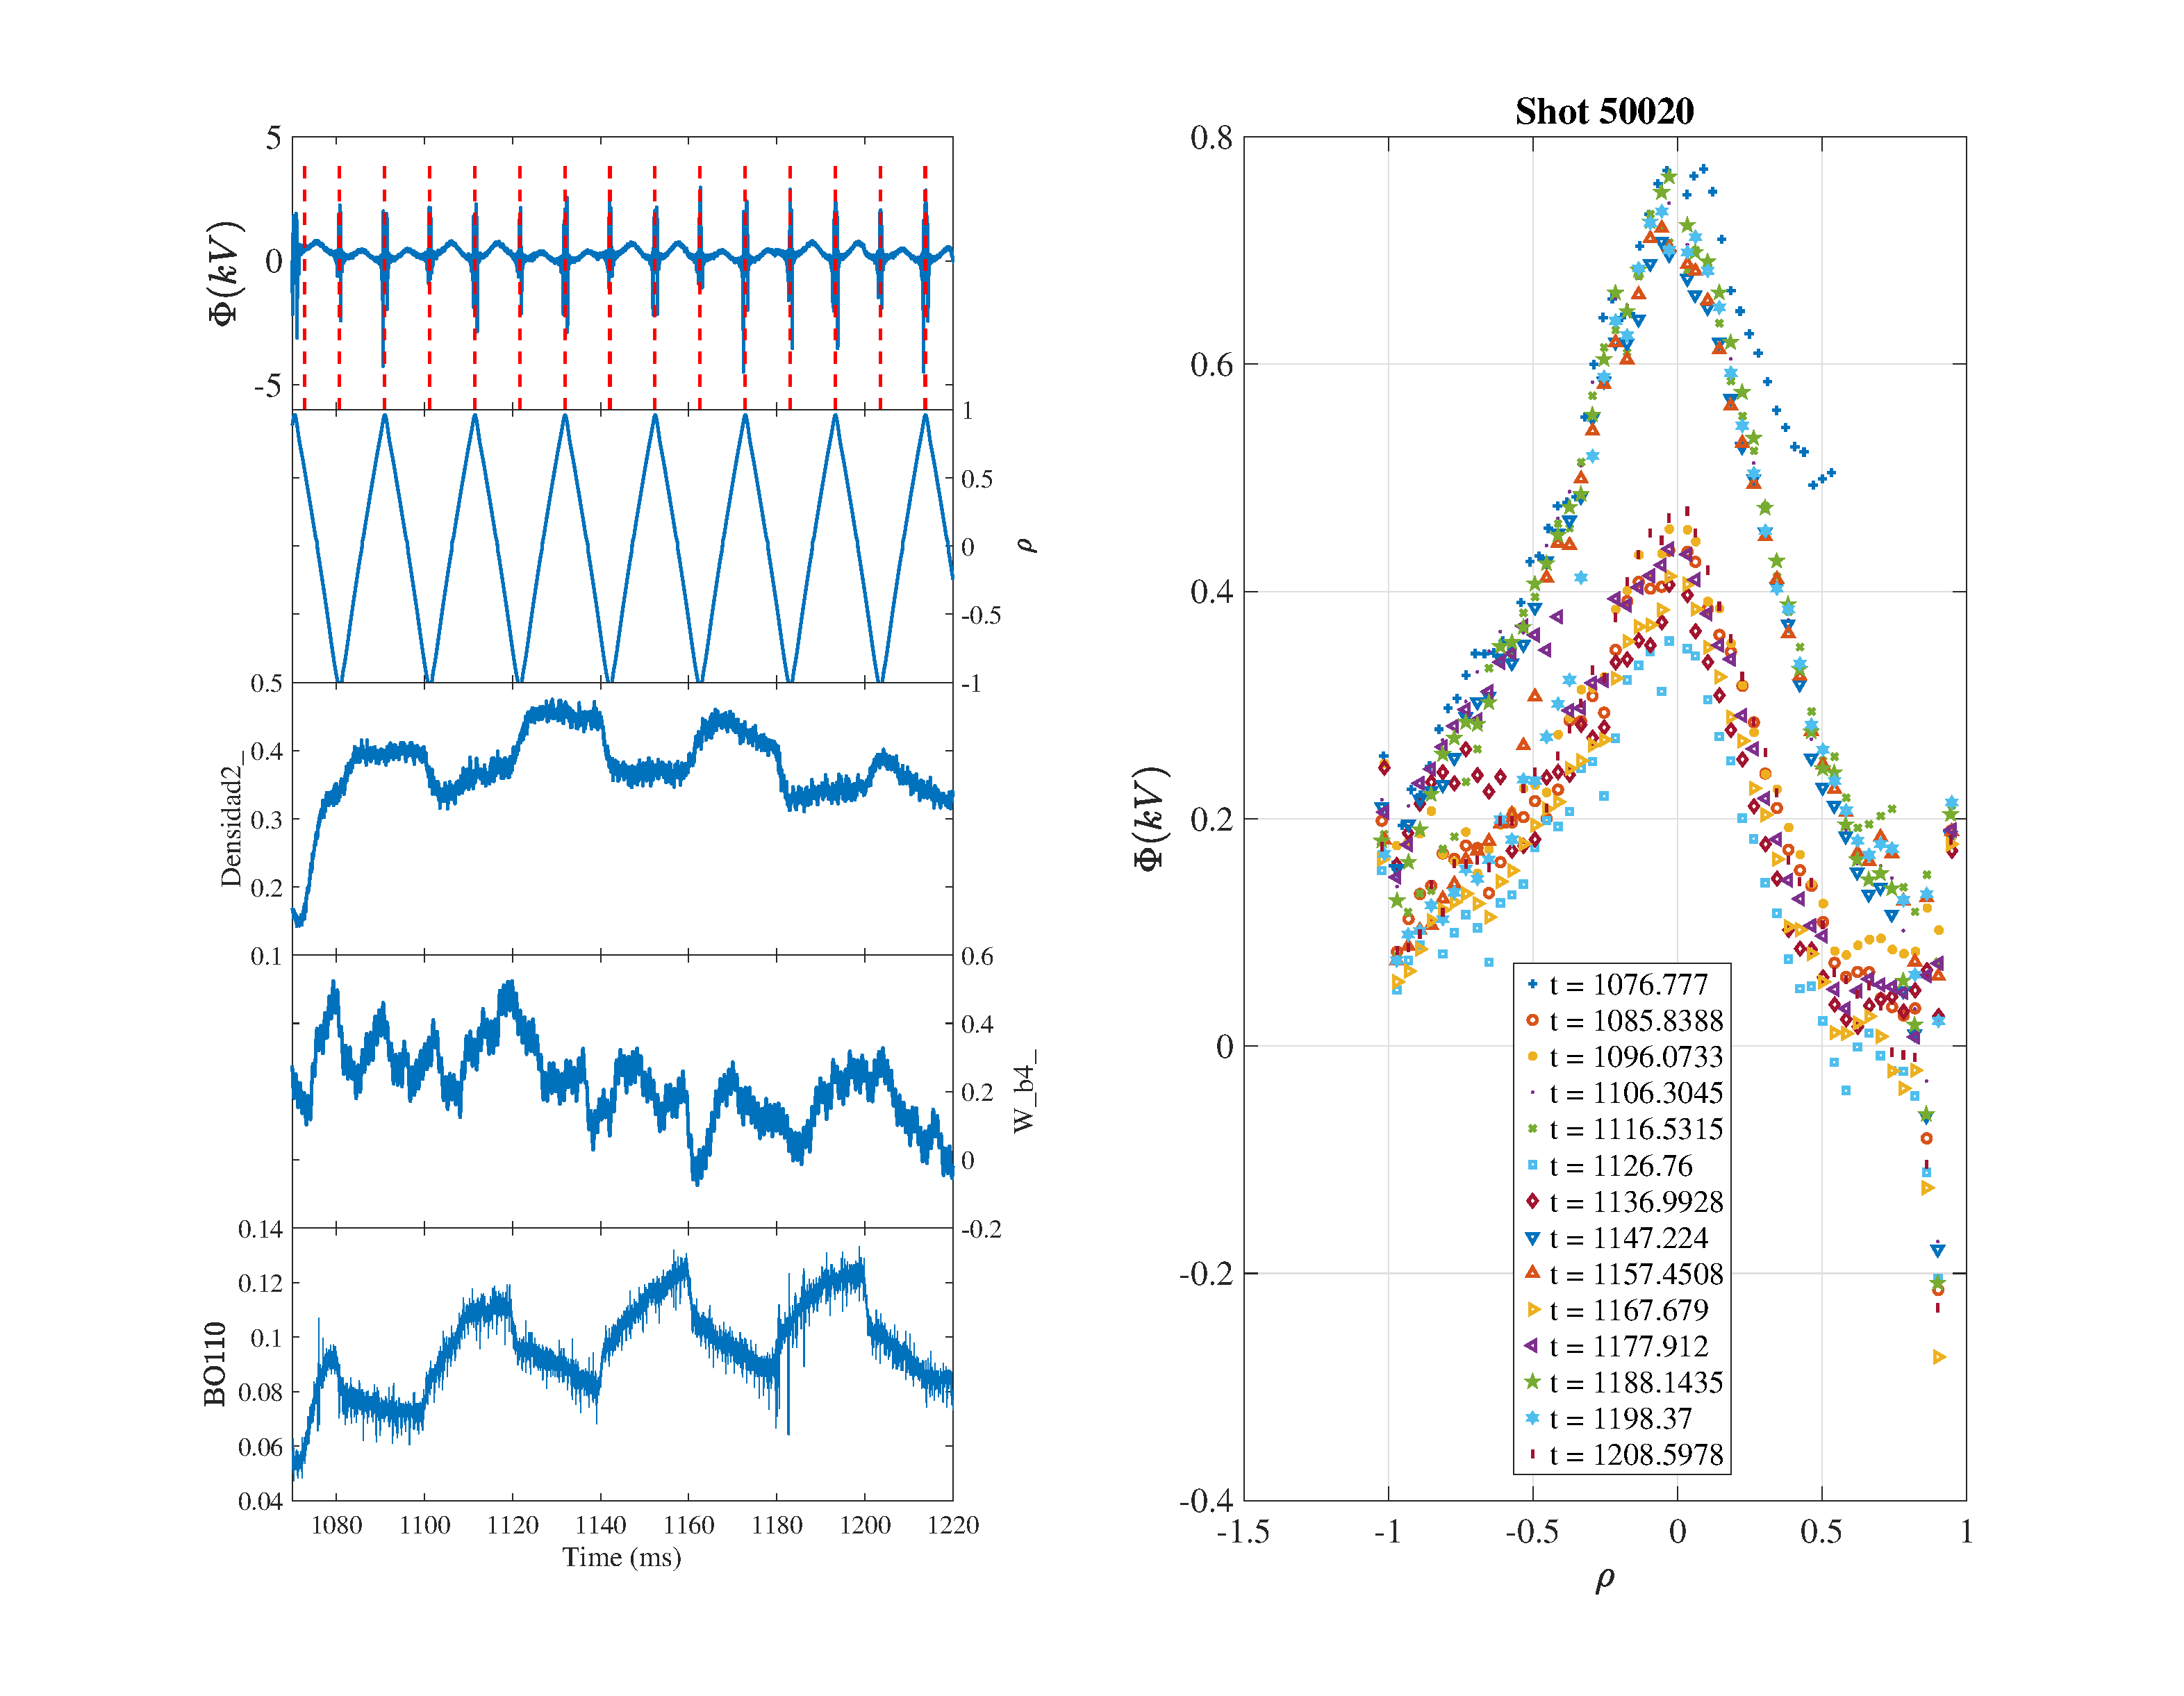
\includegraphics[width=0.9\columnwidth]{Images/HIBP_Phi.eps}
   \caption{HIBP $\Phi$ profiles for ECRH on / off (shot 50020, HIBP1). Low density case, $n_e < n_{e,c}$. The profiles basically fall in two categories. At high $P_{ECRH}$, $\Phi$ is more positive.}
   \label{Fig:HIBP_Phi}
\end{figure}

\begin{figure}[!ht]
\centering
   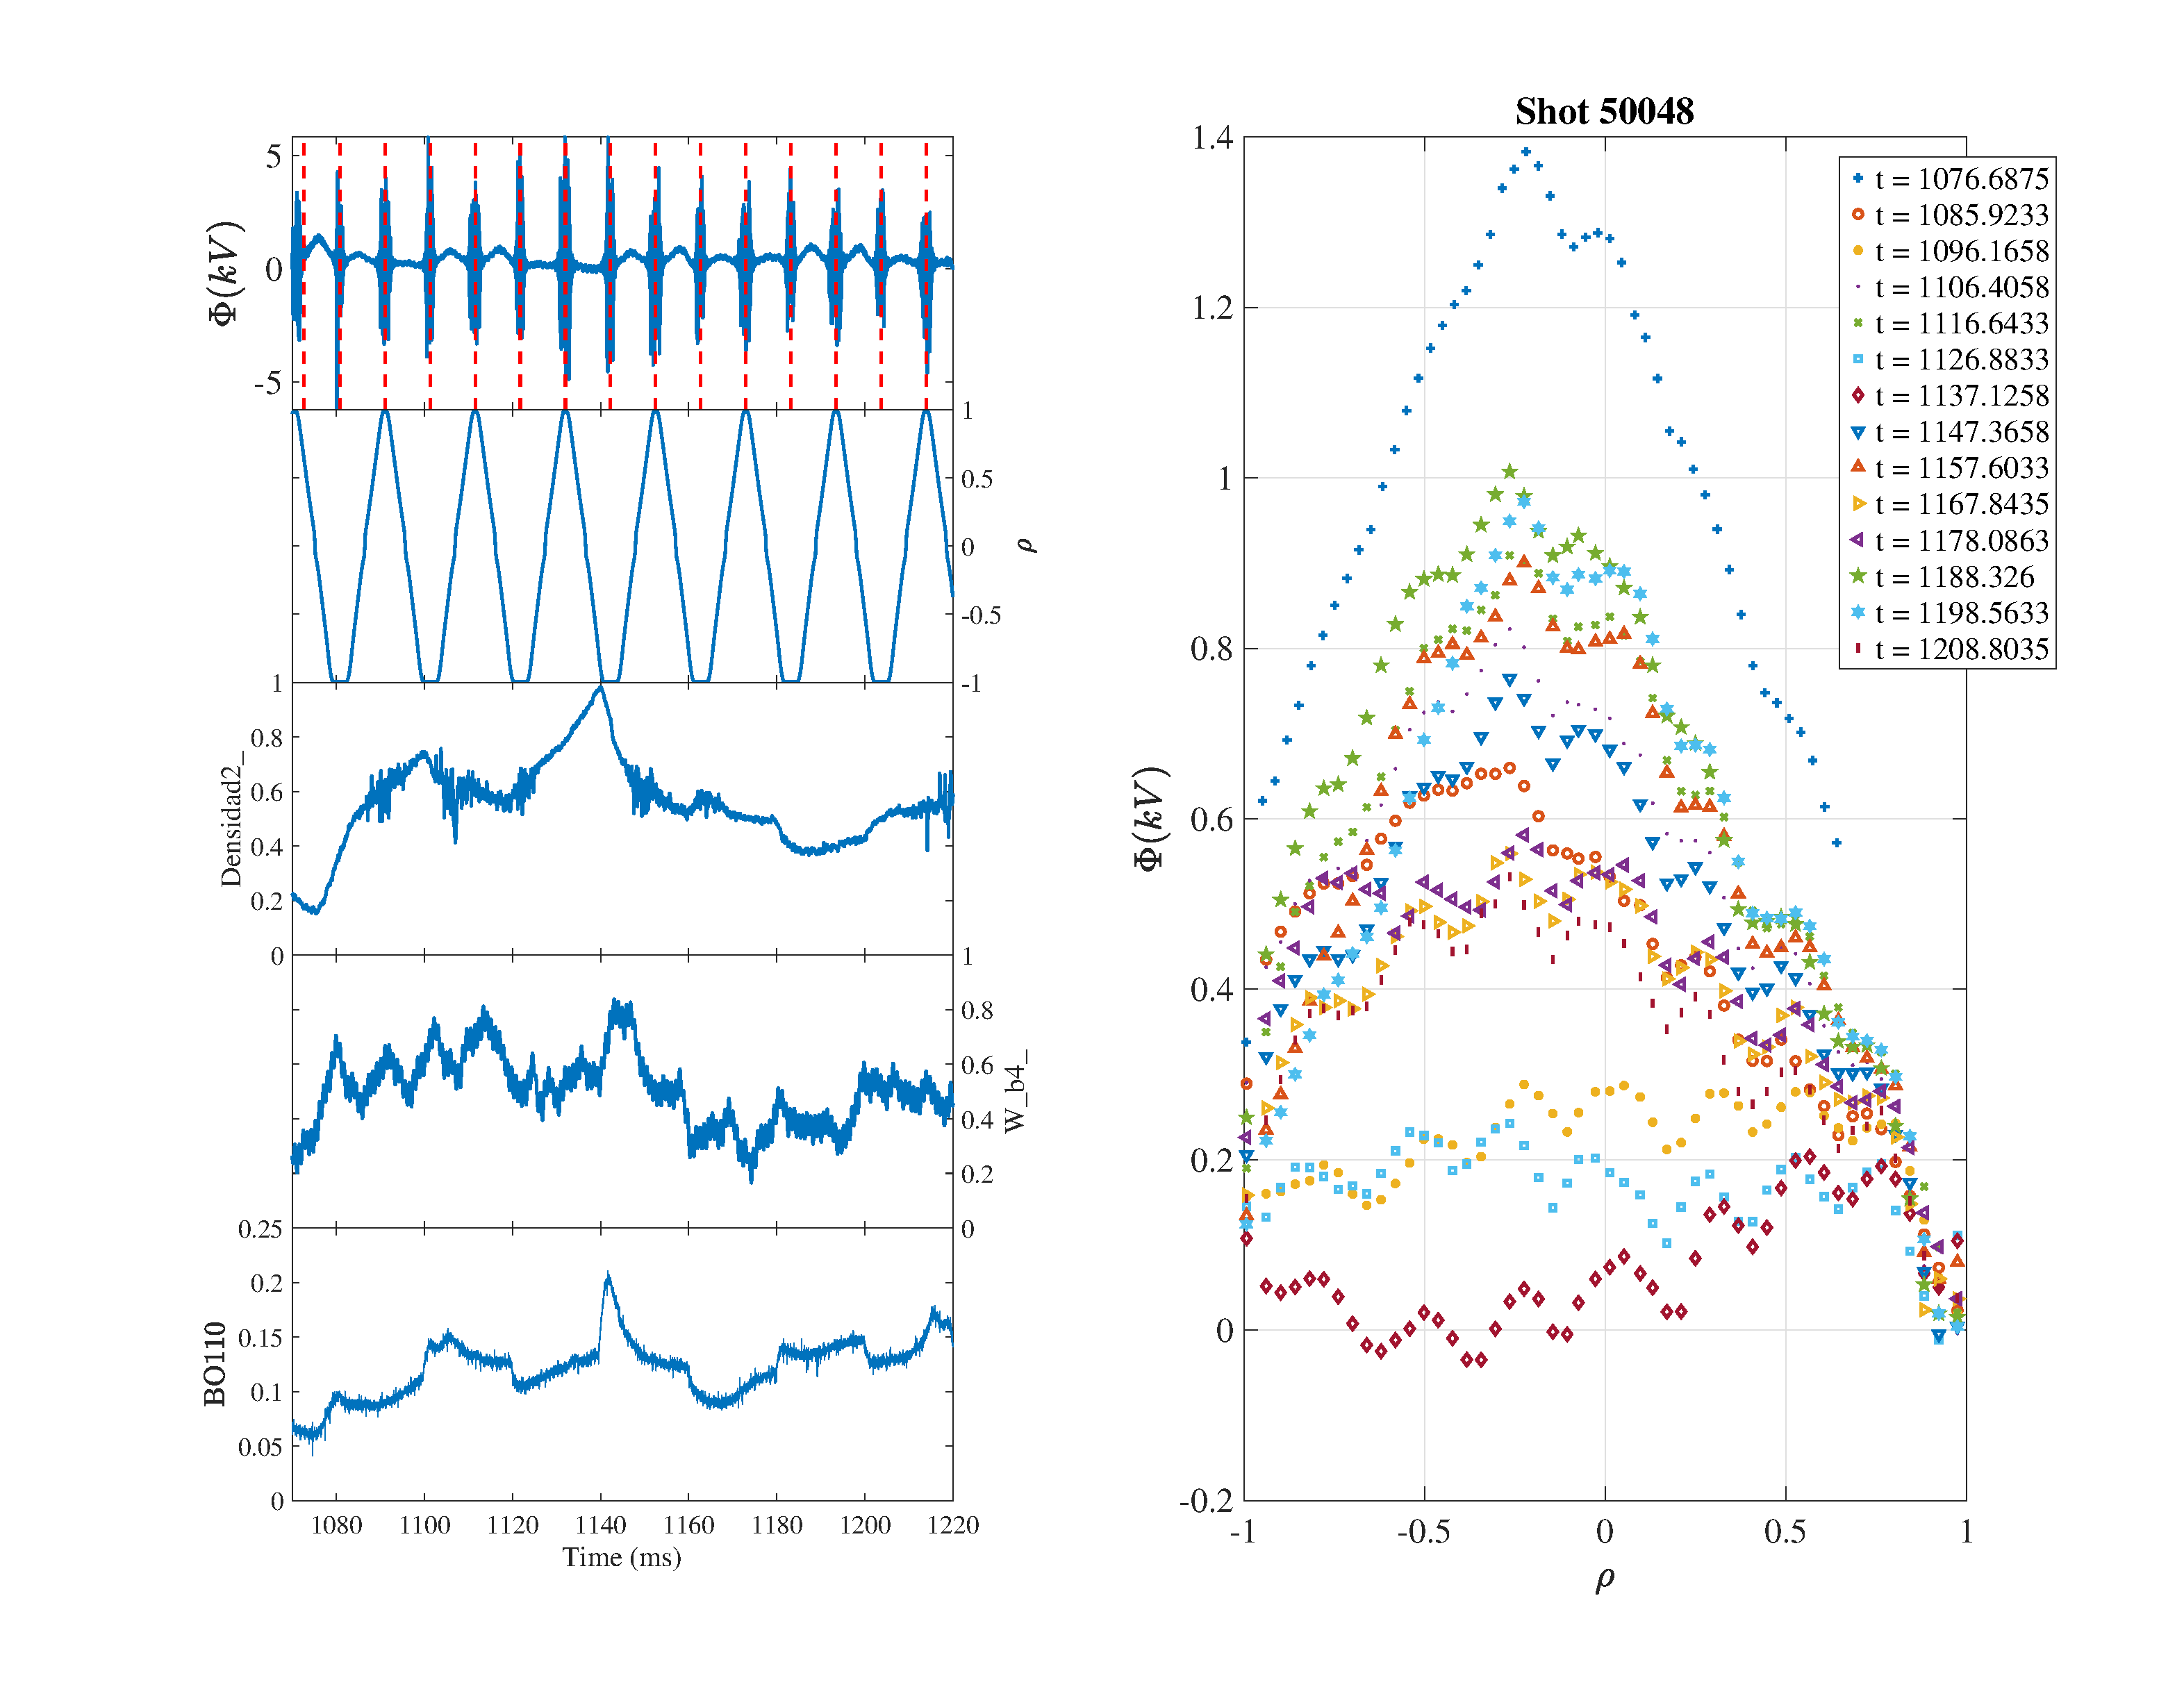
\includegraphics[width=0.9\columnwidth]{Images/HIBP_Phi2.eps}
   \caption{HIBP $\Phi$ profiles for ECRH on / off (shot 50048, HIBP2). Medium density case, $n_e \simeq n_{e,c}$. Again, the profiles basically fall in two categories. At high $P_{ECRH}$, $\Phi$ is more positive. At low $P_{ECRH}$, $\Phi$ is more negative and the profile nearly inverts. The `wiggliness' of the profiles is not real.}
   \label{Fig:HIBP_Phi2}
\end{figure}

\begin{figure}[!ht]
\centering
   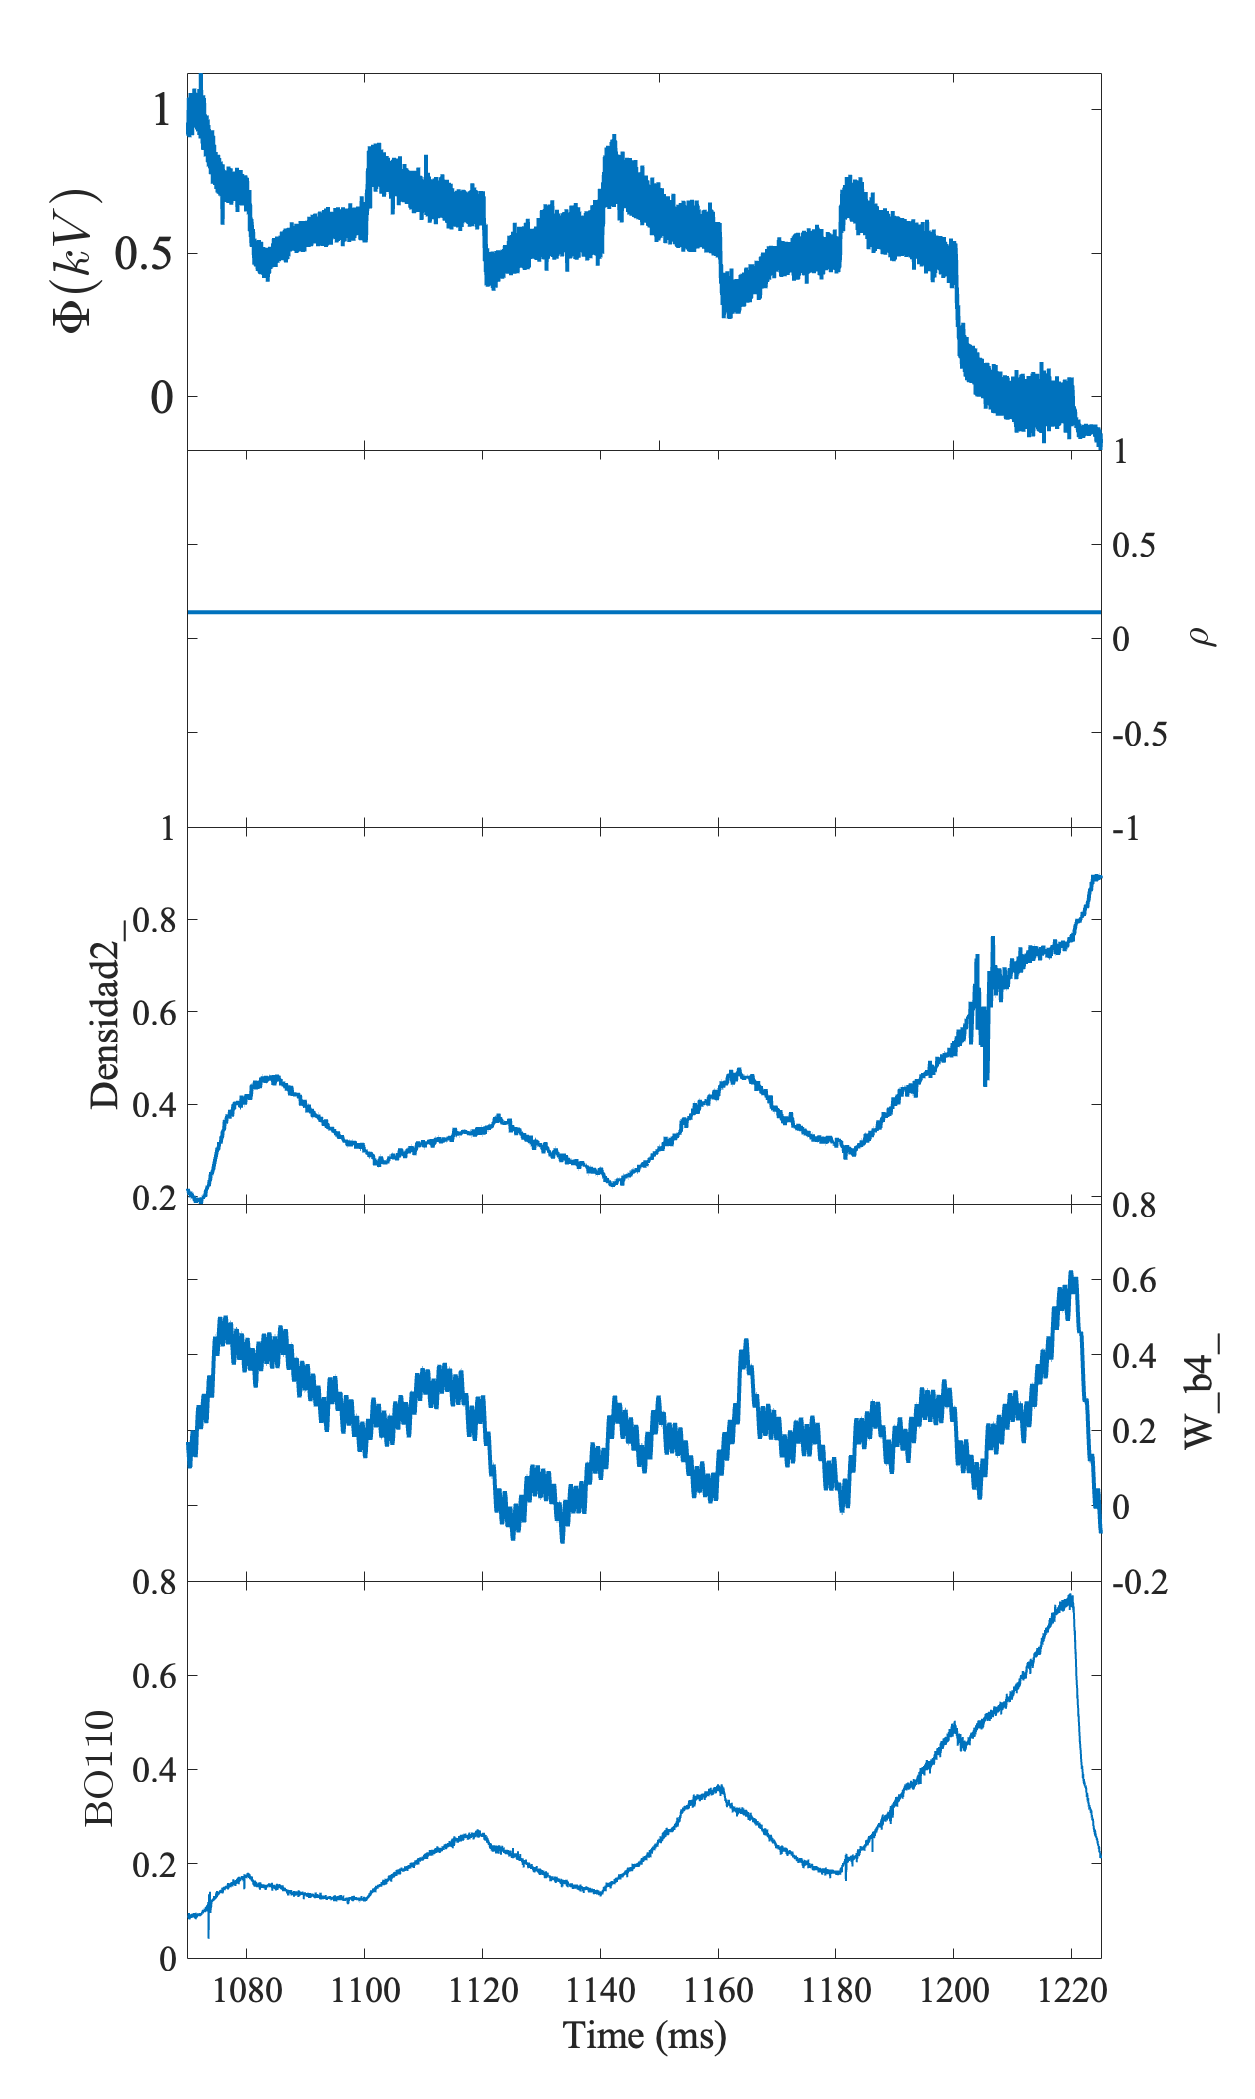
\includegraphics[width=0.7\columnwidth]{Images/HIBP_50037.png}
   \caption{HIBP time trace, shot 50037. Low $n_e$ for most of the shot, and plasma potential $\Phi$ in core responds rapidly to ECRH on/off. At $t\simeq 1200$ ms, the e to i-root transition occurs (due to increasing $n_e$), so that $\Phi$ becomes negative but on a slower timescale.}
   \label{Fig:HIBP_50037}
\end{figure}

\clearpage
\subsection{Electron Cyclotron Emission}

ECE allows following the spatiotemporal evolution $T_e(\rho,t)$ in the core plasma region, provided $n_e$
is below the cutoff density.
ECE is cross-calibrated against Thomson Scattering.
Fig. \ref{Fig:ECE} shows an example for low density; see script ECE\_analysis.m.
The temporal response to ECRH steps is fast in the core region, but slow further out.
This slow response is due to radial transport, so this observation provides an experimental measure of the transport time scale; you can fit an exponent, $A + B\exp(-(t-t_0)/\tau)$ to the curve $T_e(t)$ following an ECRH step at $t=t_0$ to obtain the time scale $\tau$.
In the core region, $\tau$ is small because the dynamics are dominated by the immediate heating response; in the edge region, $\tau$ is large because the dynamics are dominated by transport.

\begin{figure}[!ht]
\centering
   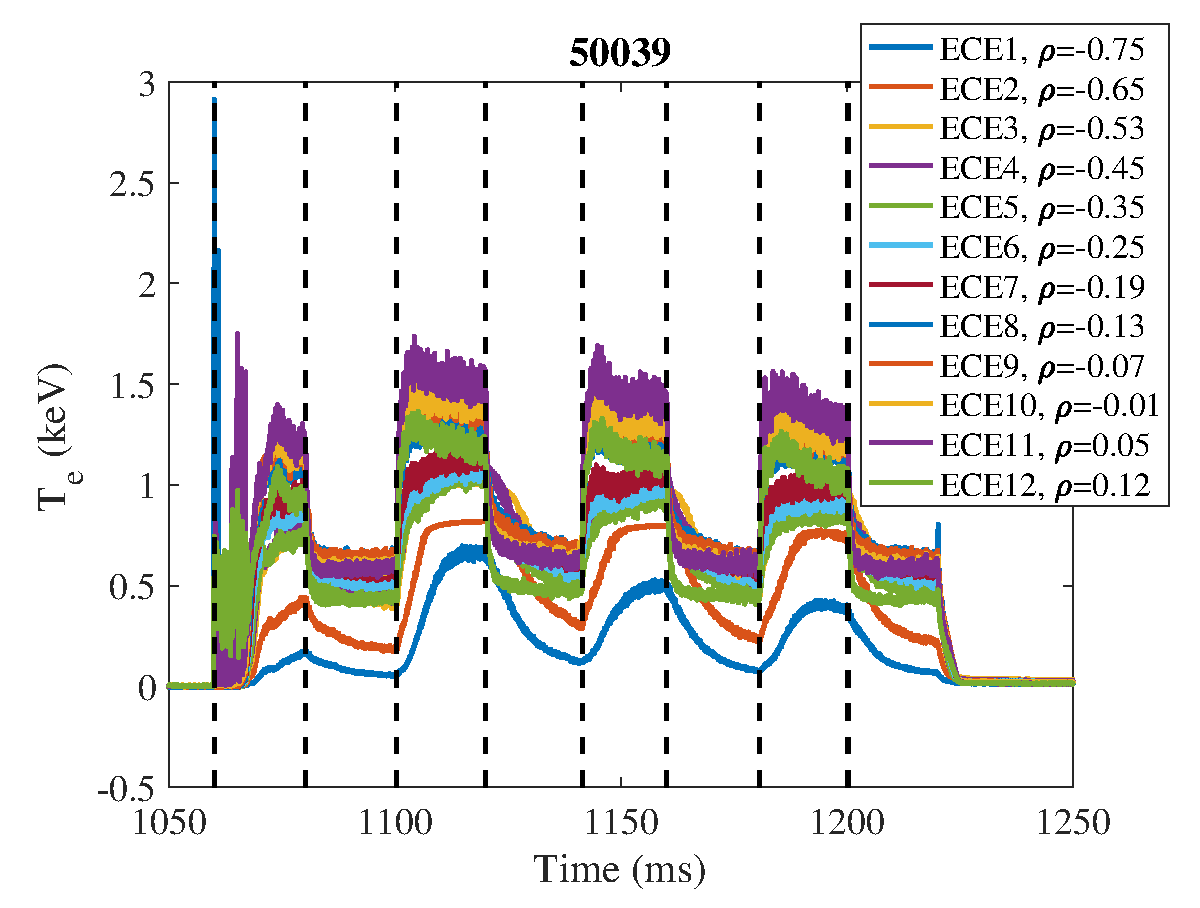
\includegraphics[width=0.9\columnwidth]{Images/ECE.eps}
   \caption{$T_e$ time traces from the ECE diagnostic. The times of ECRH switch-on and switch-off are indicated by vertical dashed lines.}
   \label{Fig:ECE}
\end{figure}

The ECRH power deposition profile can be estimated by detecting the change of slope $dT_e/dt$ immediately before and after the ECRH switching times (ignoring transport): 
$$\Delta P_{ECRH} = \Delta \left ( \frac32 \frac{d}{dt}(n_eT_e) \right ).$$ 
See Fig. \ref{Fig:ECE_deposition}.
The upward power steps yield larger changes in slope than the downward steps, as the downward steps are affected by relatively slow radial transport.
While most of the power is deposited within $\rho < 0.2$, significant power is also deposited outside the core region \cite{S_Eguilior_2003}.

NOTE: this case is off-axis ECRH (to be compared with an on-axis case). So, even with off-axis ECRH, much of the modulated power is deposited in the core, probably due to multi-pass absorption.
How much power? Can we quantify this? Maybe $P(\rho\le 0.2)/P_{tot}$, and estimate this for all shots?

\begin{figure}[!ht]
\centering
   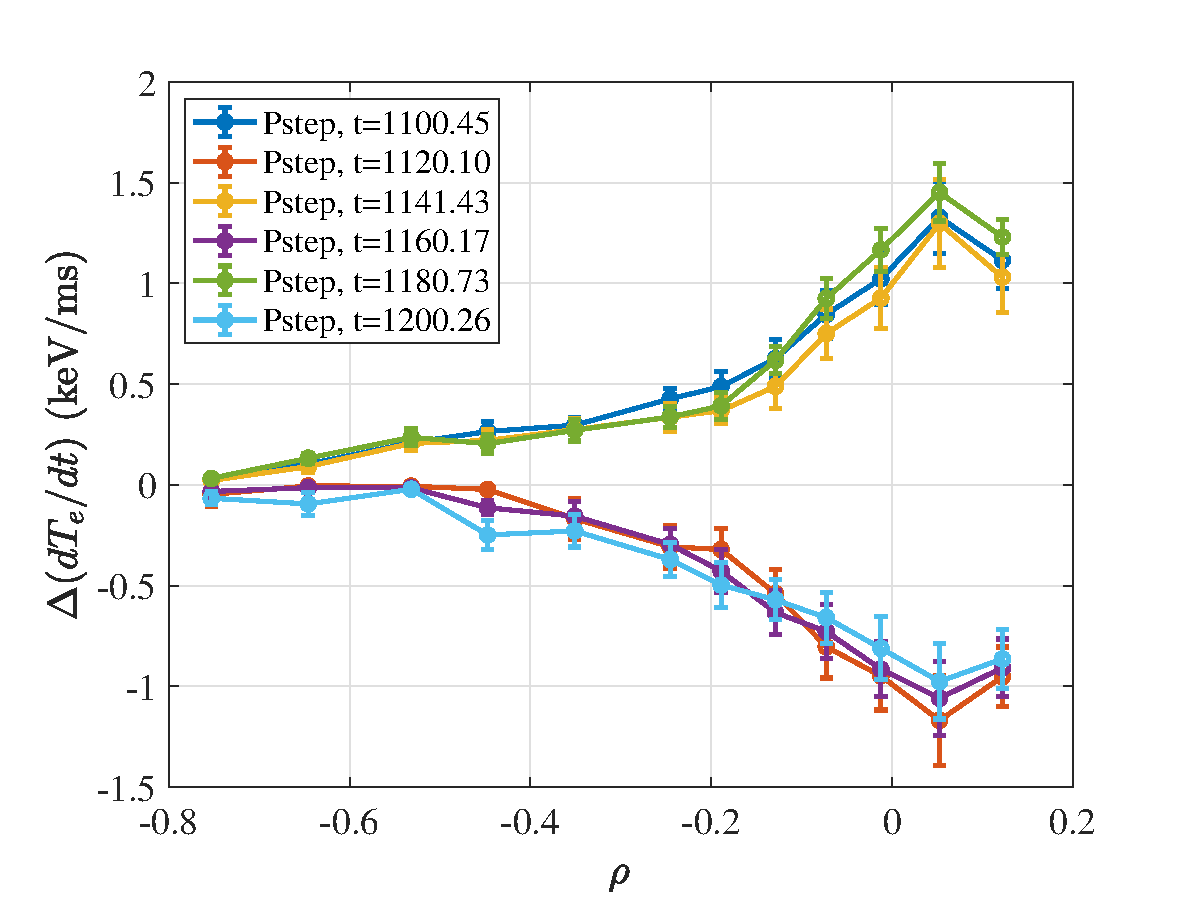
\includegraphics[width=0.5\columnwidth]{Images/ECE_power_deposition.eps}
   \caption{Change in $dT_e/dt$ across the $P_{ECRH}$ changes (up or down). Shot 50039.}
   \label{Fig:ECE_deposition}
\end{figure}

\clearpage
\subsection{Langmuir Probe profiles}

See script plot\_Langmuir.m. [NOTE LOP17 and LOP18 are `dead'.]

Fig. \ref{Fig:Langmuir_profiles} shows edge profiles for a single shot of the series ($n_e < n_{e,c}$).
The profiles are averaged over time intervals with constant $P_{ECRH}$.
When ECRH1 is on, the floating potential is higher. The ion saturation current varies by a smaller relative amount.

\begin{figure}[!ht]
\centering
   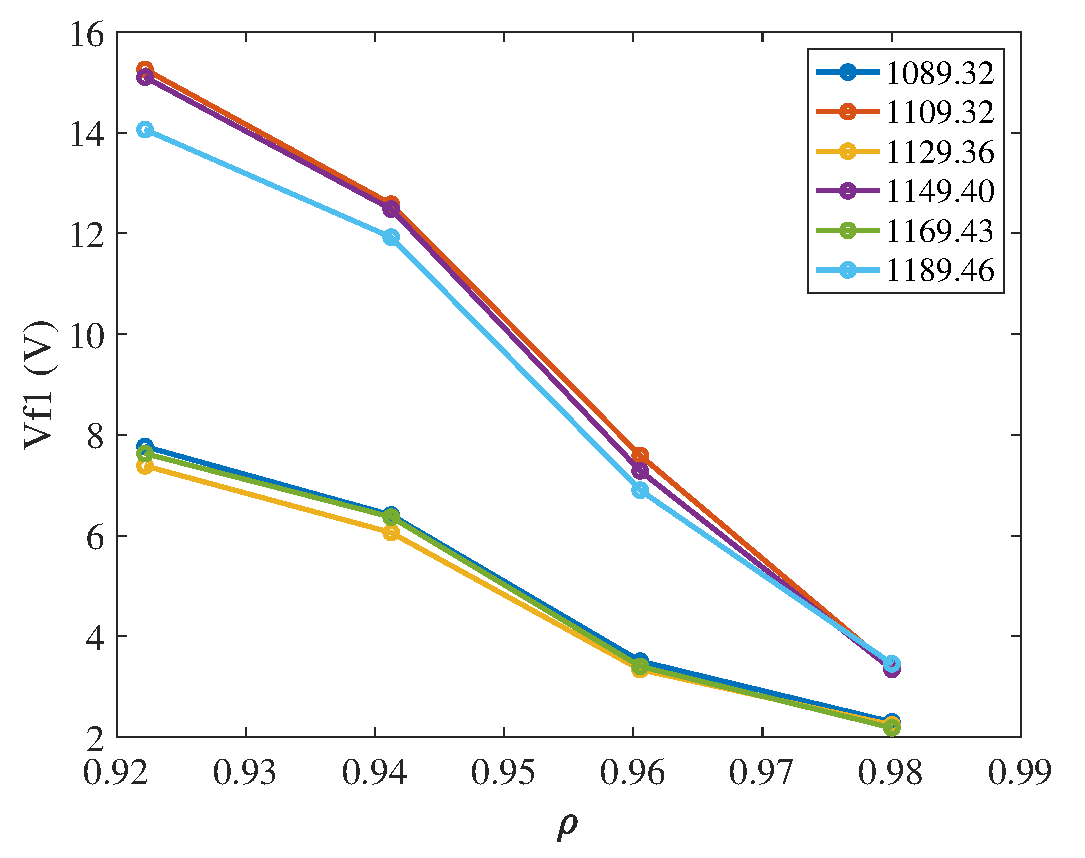
\includegraphics[width=0.32\columnwidth]{Images/50030_VF1_.eps}
   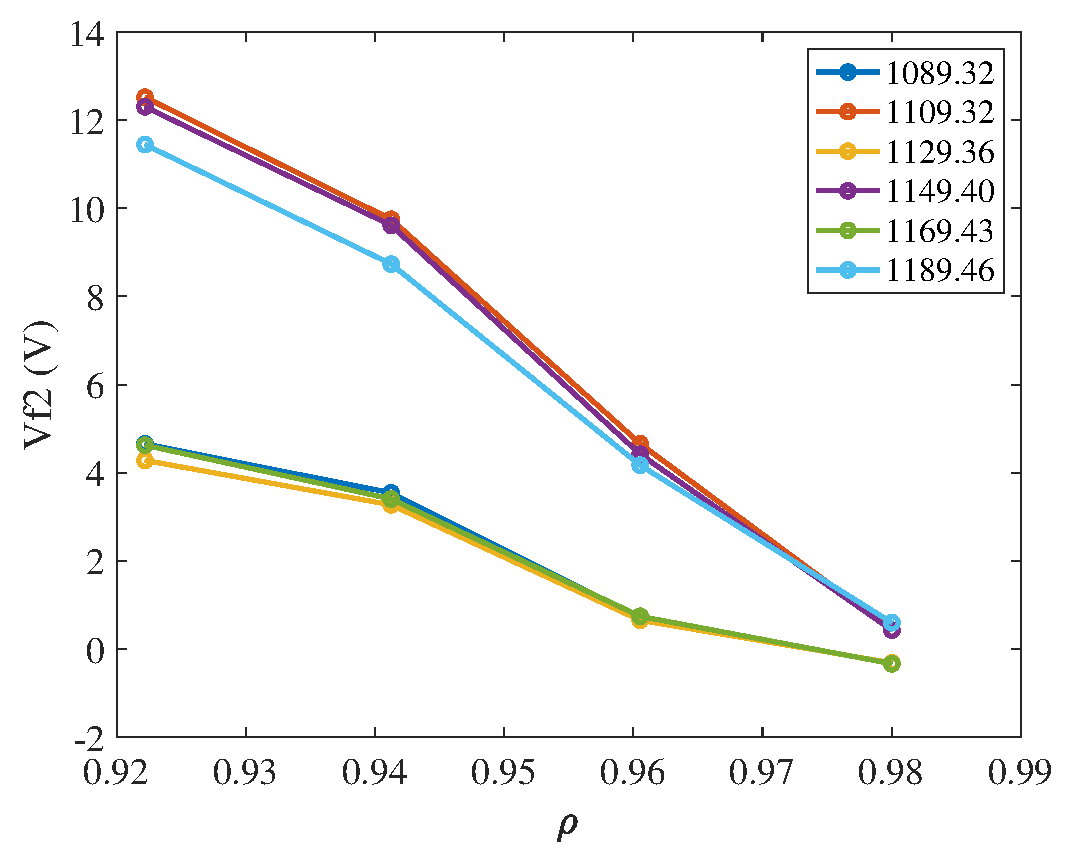
\includegraphics[width=0.32\columnwidth]{Images/50030_VF2_.eps}
   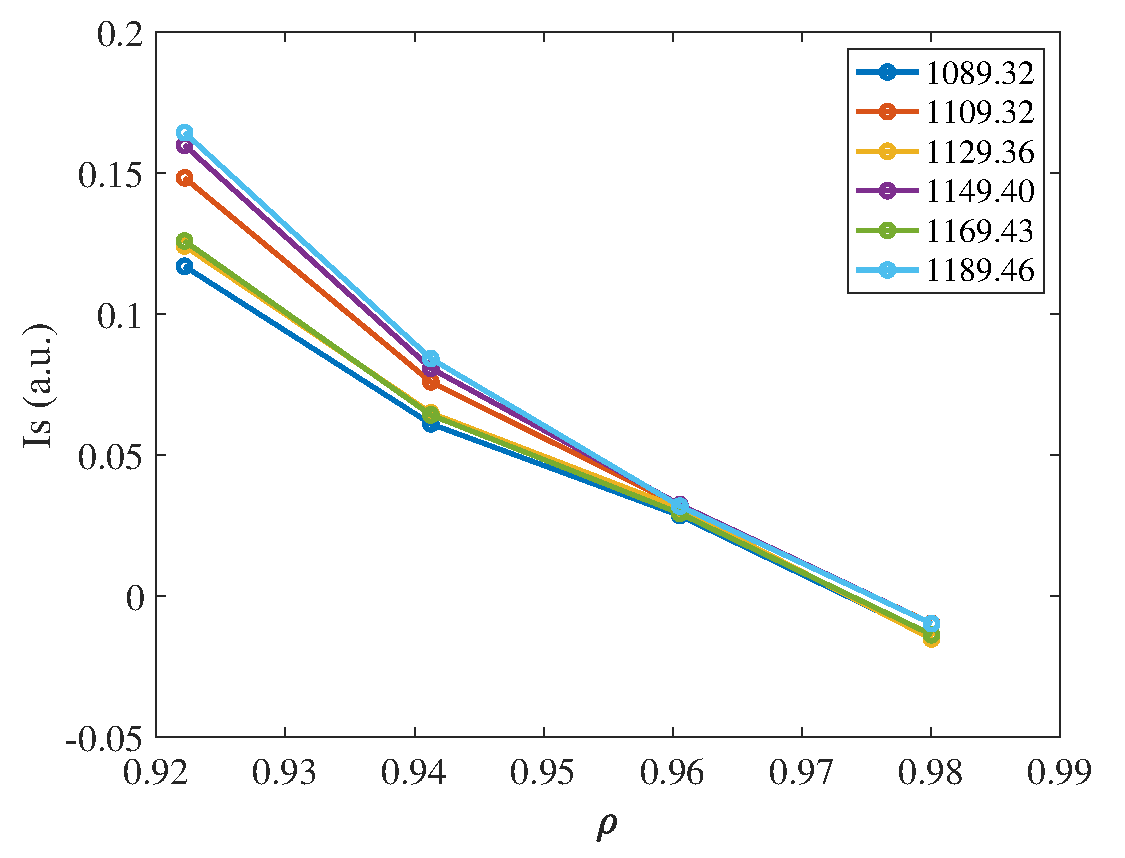
\includegraphics[width=0.32\columnwidth]{Images/50030_Is_.eps}
   \caption{Langmuir profiles for shot 50030.}
   \label{Fig:Langmuir_profiles}
\end{figure}

Fig. \ref{Fig:Langmuir_RMSprofiles} shows edge profiles of the RMS (fluctuation amplitude) for a single shot of the series ($n_e < n_{e,c}$).
The profiles are averaged over time intervals with constant $P_{ECRH}$.
The RMS does not vary as $P_{ECRH}$ is varied.

\begin{figure}[!ht]
\centering
   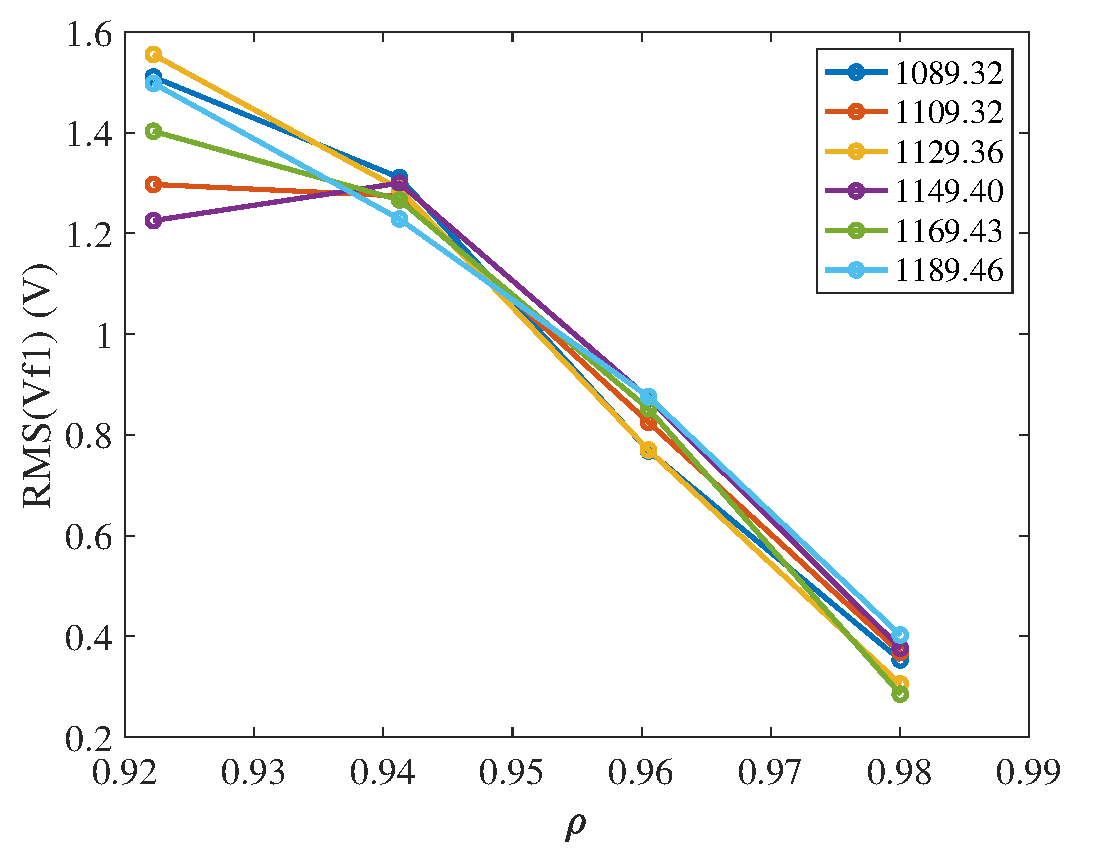
\includegraphics[width=0.32\columnwidth]{Images/50030_VF1_RMS.eps}
   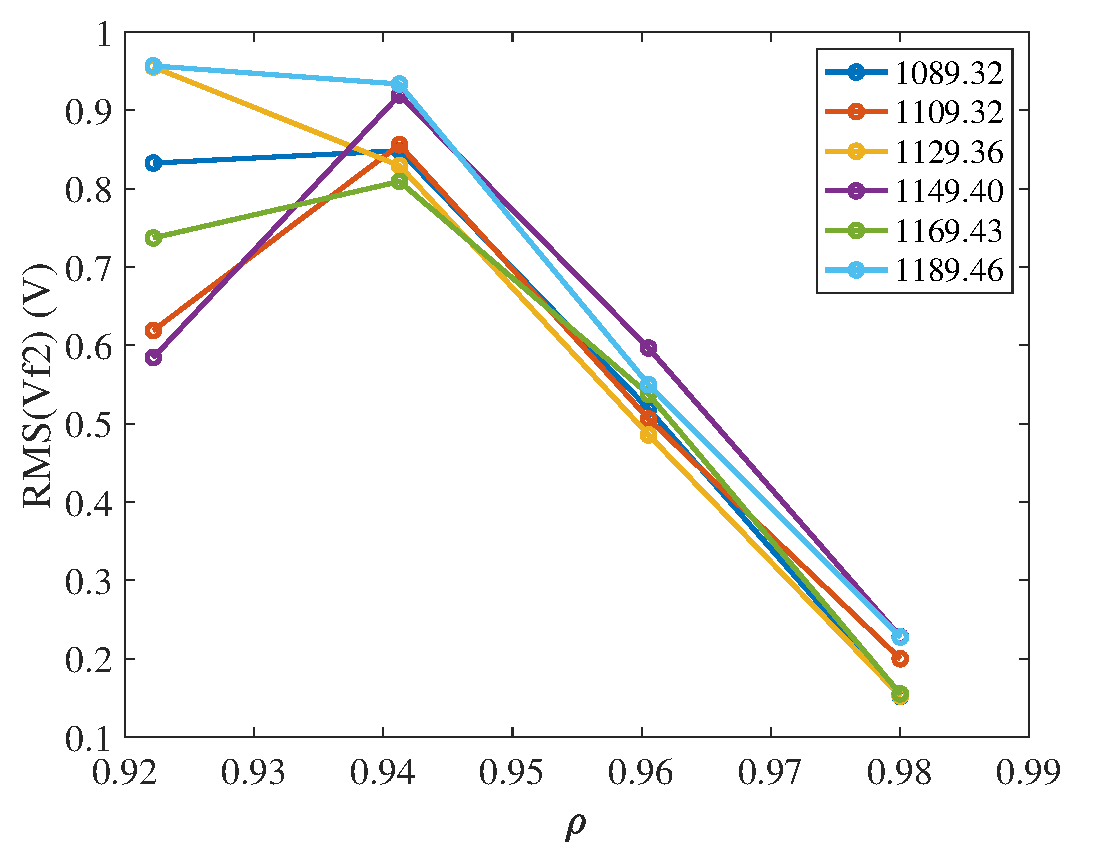
\includegraphics[width=0.32\columnwidth]{Images/50030_VF2_RMS.eps}
   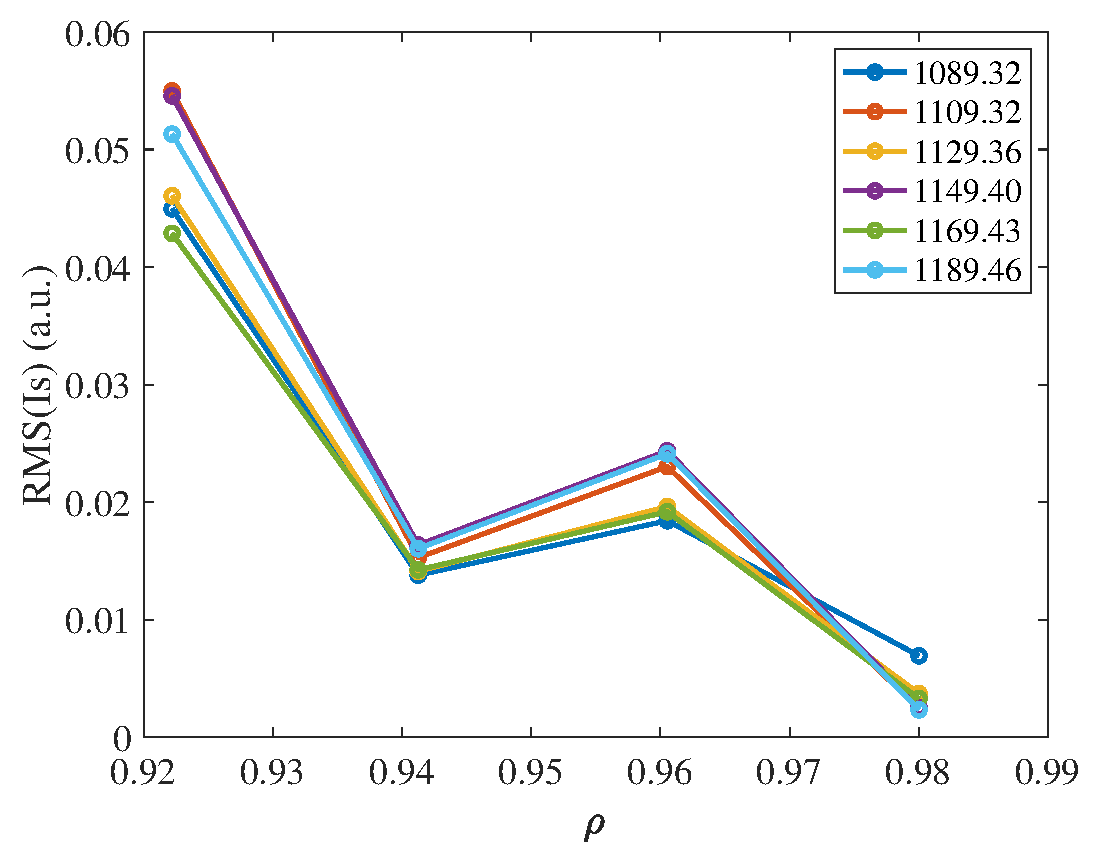
\includegraphics[width=0.32\columnwidth]{Images/50030_Is_RMS.eps}
   \caption{Langmuir RMS profiles for shot 50030.}
   \label{Fig:Langmuir_RMSprofiles}
\end{figure}

Fig. \ref{Fig:Langmuir_profiles1} shows edge profiles for another shot of the series ($n_e < n_{e,c}$).
The profiles are averaged over time intervals with constant $P_{ECRH}$.
When ECRH1 is on, the floating potential is higher. The ion saturation current varies by a smaller relative amount.
Density $n_e$ is gradually increasing, leading to a gradual reduction of $V_f$.

\begin{figure}[!ht]
\centering
   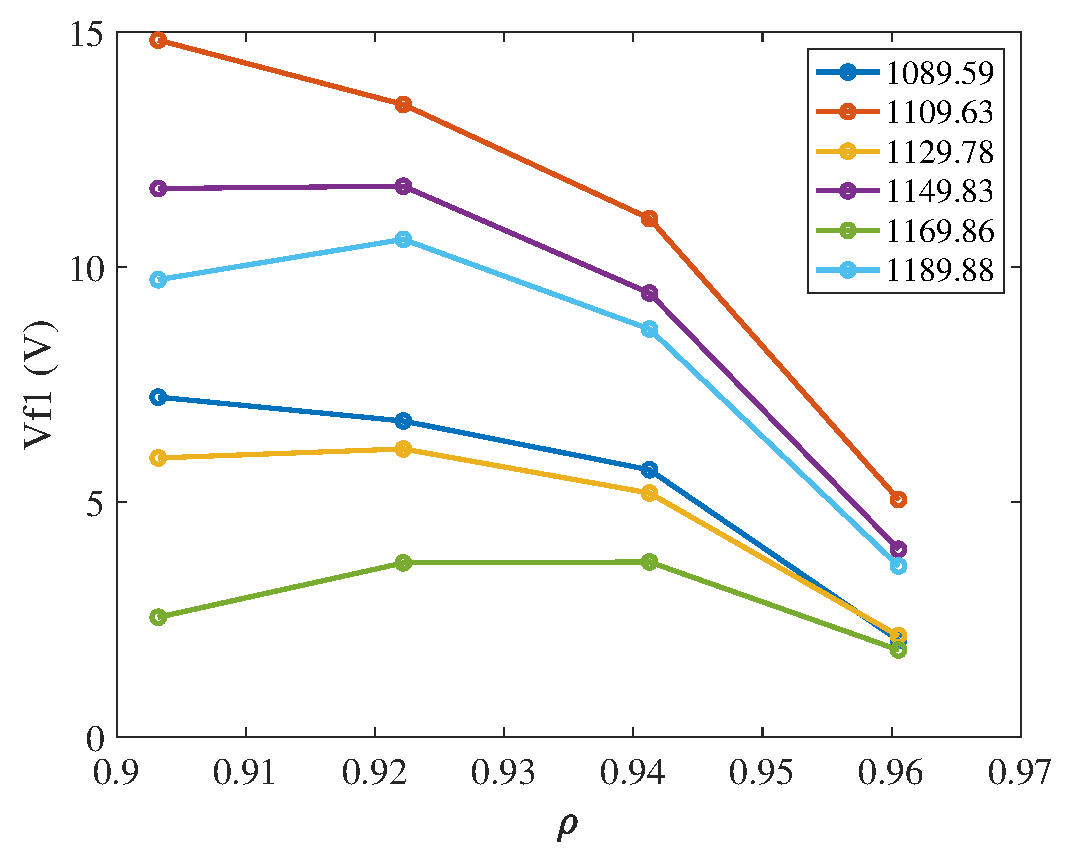
\includegraphics[width=0.32\columnwidth]{Images/50031_VF1_.eps}
   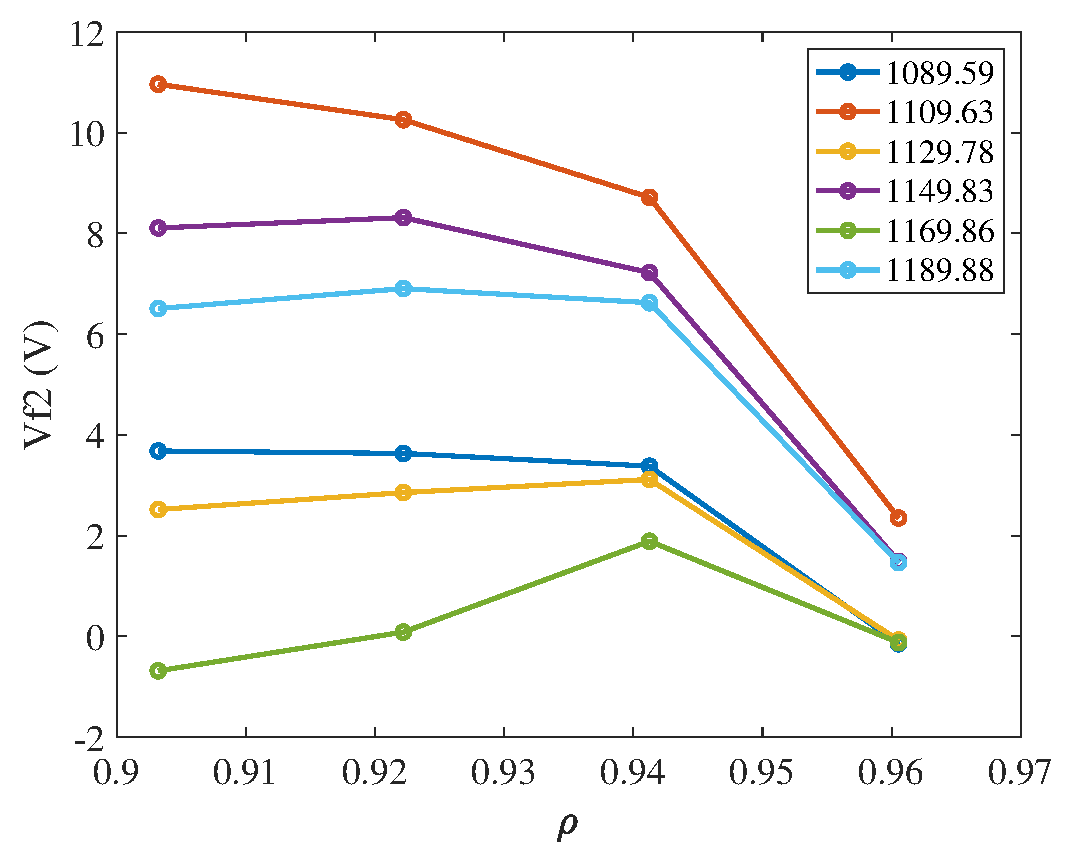
\includegraphics[width=0.32\columnwidth]{Images/50031_VF2_.eps}
   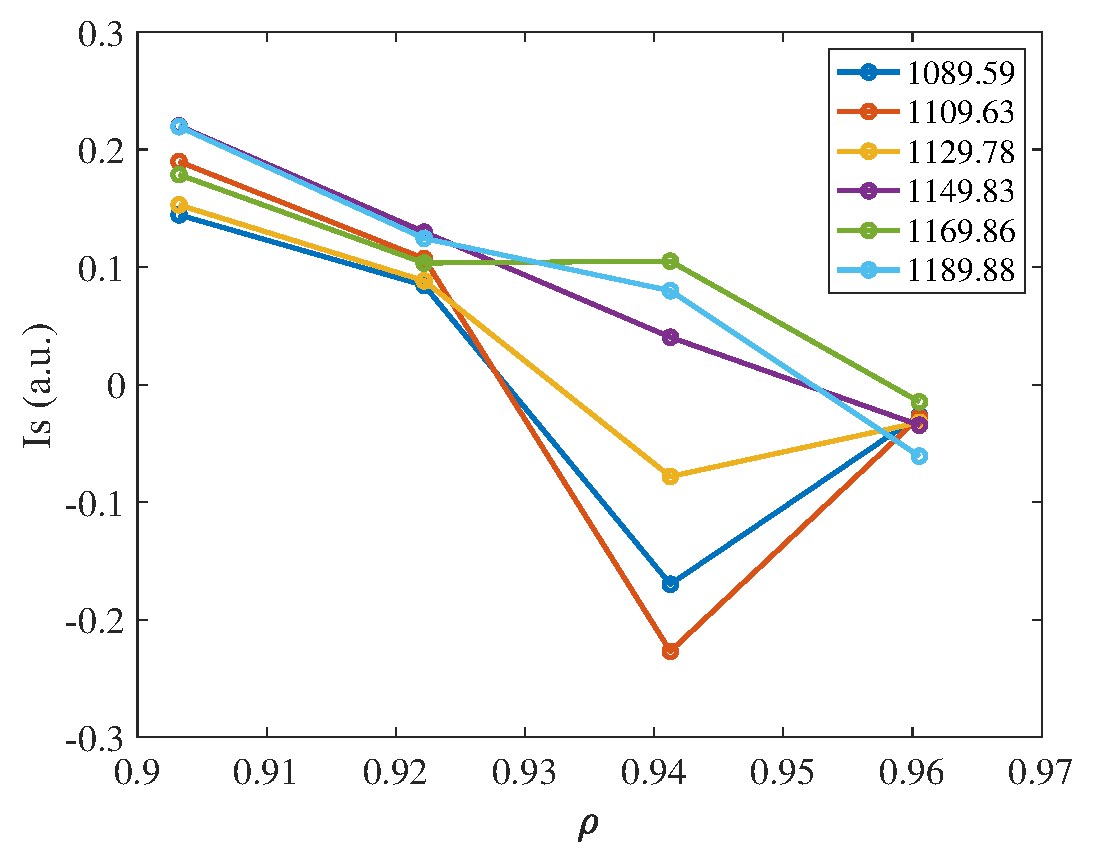
\includegraphics[width=0.32\columnwidth]{Images/50031_Is_.eps}
   \caption{Langmuir profiles for shot 50031.}
   \label{Fig:Langmuir_profiles1}
\end{figure}

Fig. \ref{Fig:Langmuir_RMSprofiles1} shows edge profiles of the RMS (fluctuation amplitude) for a single shot of the series ($n_e < n_{e,c}$).
The profiles are averaged over time intervals with constant $P_{ECRH}$.
Now a variation of RMS is seen, increasing as the density $n_e$ increases.
So: when the density approaches the critical density $n_{e,c}$, the edge turbulence amplitude increases.
(Increasing turbulence amplitude is a prelude to the formation of sheared flow at the critical density!)

\begin{figure}[!ht]
\centering
   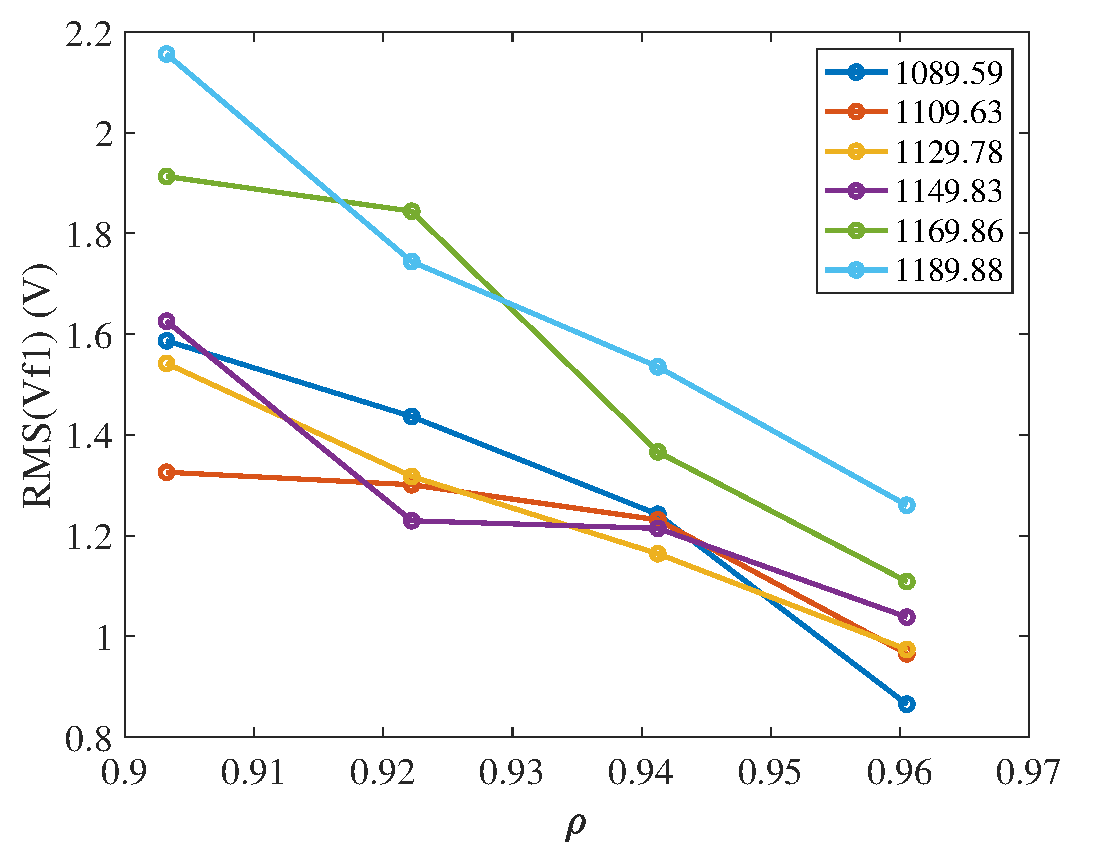
\includegraphics[width=0.32\columnwidth]{Images/50031_VF1_RMS.eps}
   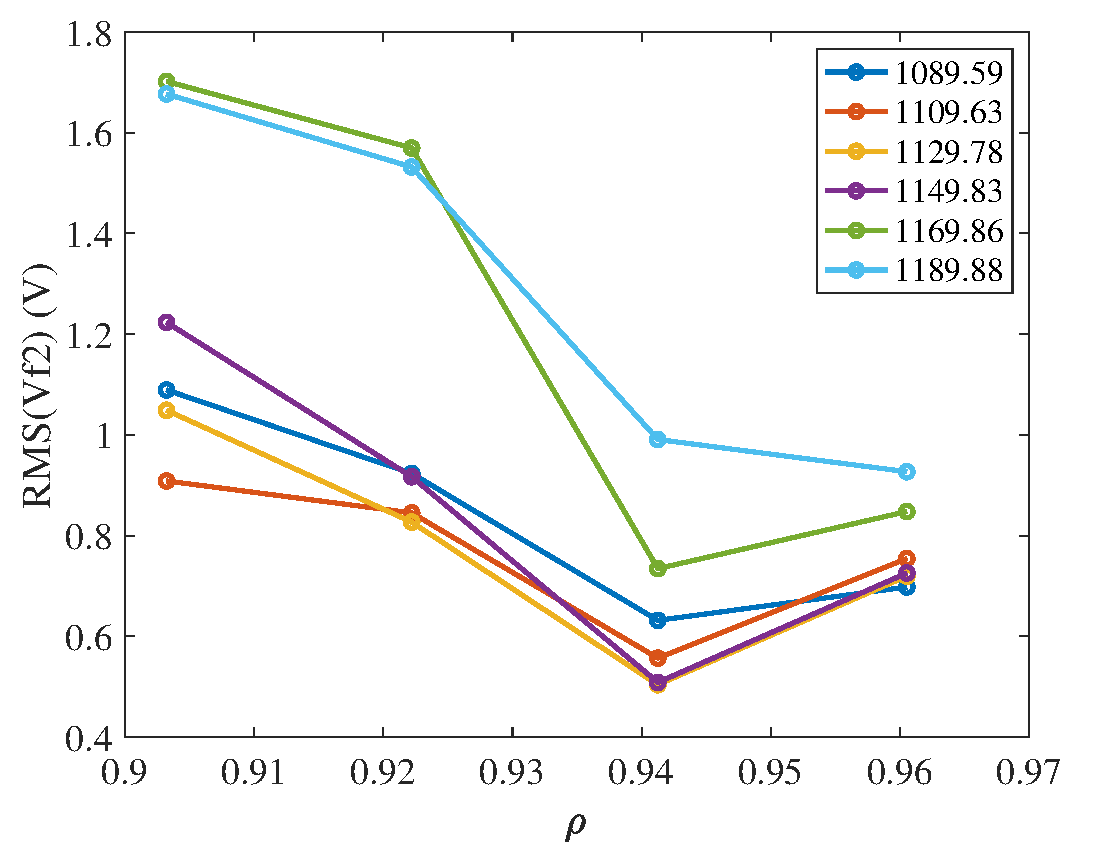
\includegraphics[width=0.32\columnwidth]{Images/50031_VF2_RMS.eps}
   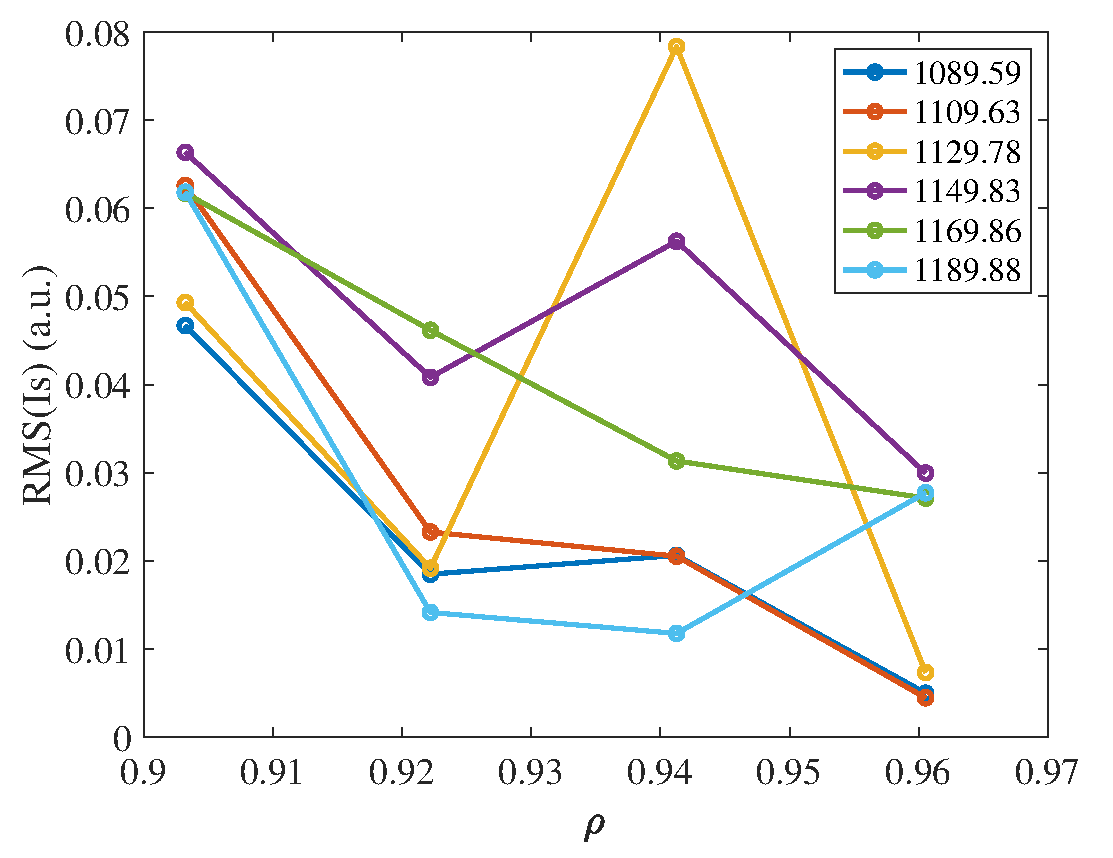
\includegraphics[width=0.32\columnwidth]{Images/50031_Is_RMS.eps}
   \caption{Langmuir RMS profiles for shot 50031.}
   \label{Fig:Langmuir_RMSprofiles1}
\end{figure}

To be done: profiles of Reynolds Stress, Intermittence, ...

Idea for analysis: create a database of these profiles, for each shot and each ECRH modulation interval. Then one can see more clearly and systematically how the profiles respond to $n_e(t)$ and $P_{ECRH}$. 

\begin{figure}[!ht]
    \centering
    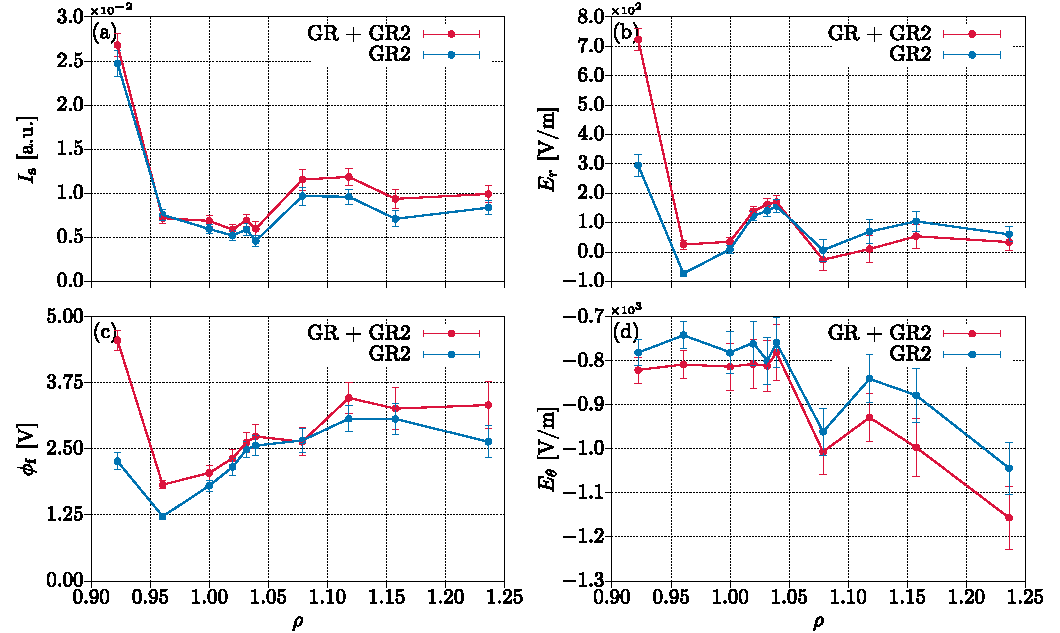
\includegraphics[width=1.0\linewidth]{Images/Rake_D_low_density.pdf}
    \caption{Radial profiles of (a) Ion saturation current $I_{s}$, (b) radial electric field $E_{r}$, (c) floating potential $\phi_{f}$ and (d) poloidal electric field $E_{\theta}$.}
    \label{Fig:Rake_D_low_density}
\end{figure}



\subsection{Turbulence}

Characterize turbulence for both heating phases (ECRH on/off), for all classes of mean $n_e$ above. Use all methods available, insofar as they yield significant results.

\begin{figure}[!ht]
    \centering
    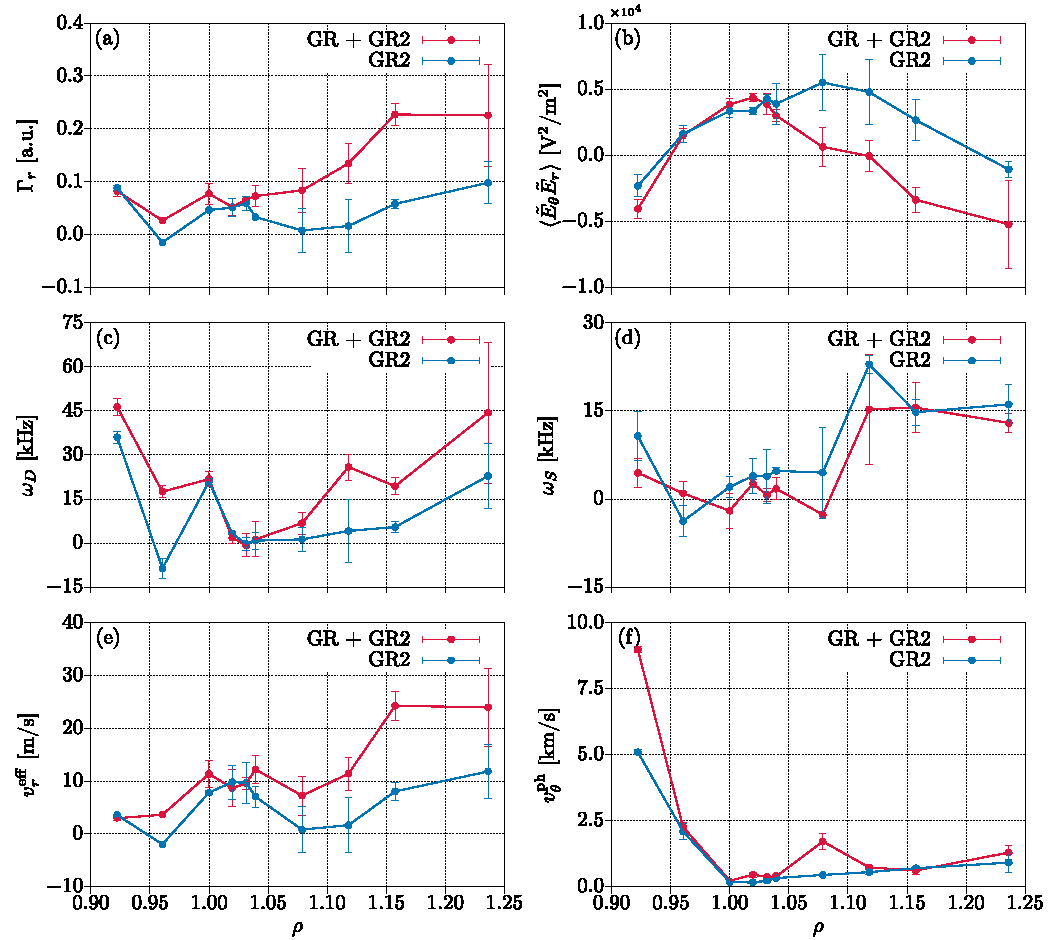
\includegraphics[width=1.0\linewidth]{Images/Rake_D_low_density_2.pdf}
    \caption{Radial profiles of (a) turbulent radial transport $\Gamma_{r}$, (b) approximation of Reynolds stress value ,(c) rate of turbulence drive $\omega_D$, (d) rate of turbulence spreading $\omega_S$, and (e) radial effective velocity $v^{\mathrm{eff}}_{r}$.}
    \label{Fig:Rake_D_low_density_2}
\end{figure}
\subsection{Long Range Correlations}

Long Range Correlations (LRCs) are a measure of either Zonal Flows or filaments \cite{Milligen:2013b}. 
In this section, we will study how the LRC varies with (a) line average density and (b) $P_{ECRH}$.
(See script correlation\_Langmuir.m).
Fig. \ref{Fig:Langmuir_LRC} shows an example for a specific shot with $n_e < n_{e,c}$. 
The LRCs change systematically with $P_{ECRH}$ (times correspond to ECRH on/off; improve plot labeling). Note: check signal contamination (spikes in correlation $C(\Delta t)$, probably due to some low frequency oscillations in the range 1-10 kHz; of course LRCs are due to precisely that: low frequency oscillations).

\begin{figure}[!ht]
\centering
   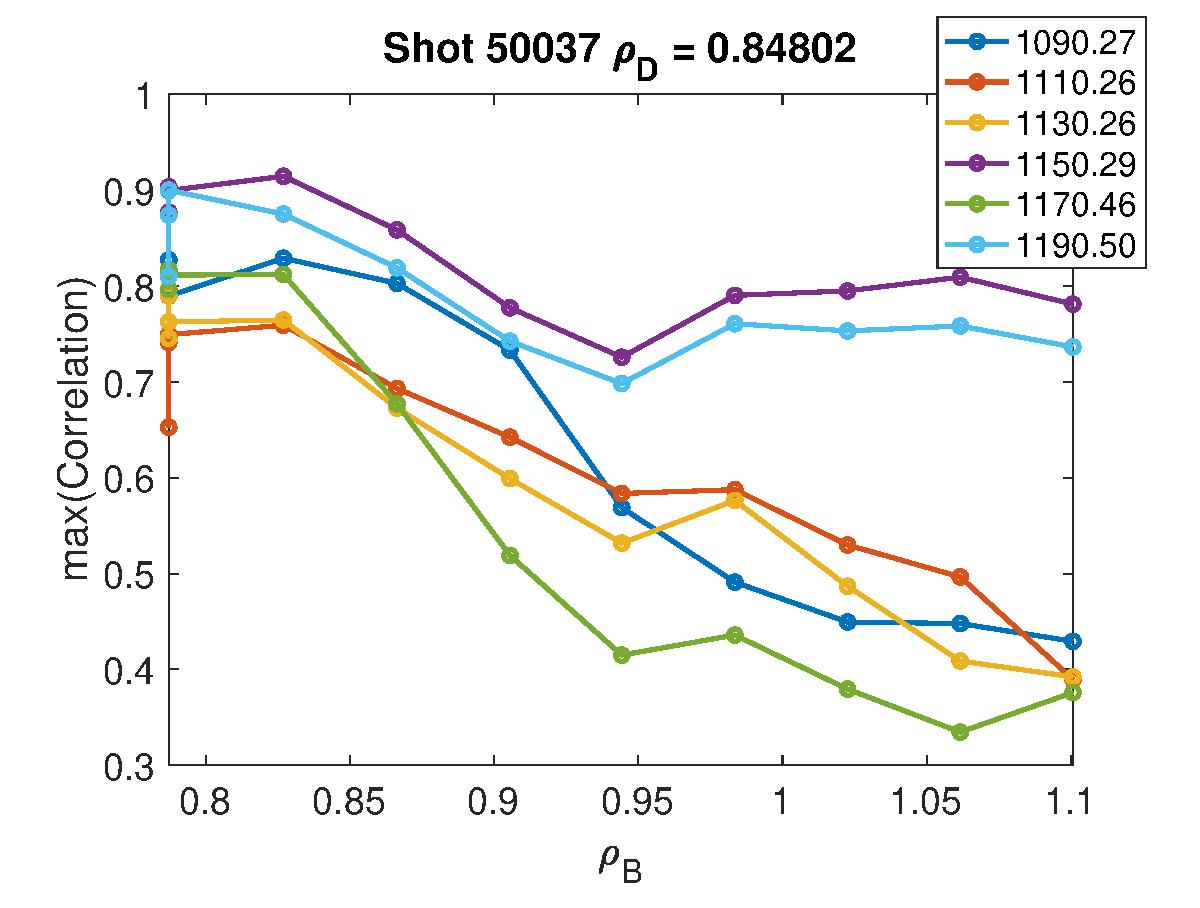
\includegraphics[width=0.75\columnwidth]{Images/50037_LRC.eps}
   \caption{Long Range Correlation between a pin from probe D and all pins from probe B. The highest correlation occurs when the pins of probes B and D are roughly at the same radial position (here, $\rho \simeq 0.85$).}
   \label{Fig:Langmuir_LRC}
\end{figure}

\subsection{Transitions}

Present a separate analysis of what happens immediately after ECRH switching times. How fast do changes occur? How do the changes propagate radially? 

\section{Discussion}

Observation: $n_e \le n_{e,c}$: the density variation is {\em in phase opposition} with the modulation of $P_{ECRH}$. 
But in two cases with $n_e > n_{e,c}$, the density variation is {\em in phase} with the modulation of $P_{ECRH}$ (off-axis).

The modulation of $n_e$ at low $n_e$ is probably (partly) a NeoClassical effect \cite{Velasco:2012}: an increase of $P_{ECRH}$ leads to an increase of $\nabla T_e$, so that the ambipolar solution to the transport equations changes, leading to a variation in $n_e$. This effect works on the time scale of {\em transport} (i.e., it's slow, requiring several ms for changes to take effect).
The following paper may provide a means to estimate the profile evolution: \cite{Gutierrez-Tapia:2015}.
We can discuss this with Victor Tribaldos once we have documented the relevant discharges (profiles).

Also note the existence of the so-called `pump-out effect': at high $P_{ECRH}$, more ripple-trapped electrons are driven into the loss cone, thus leading to a reduction of electron density at higher power \cite{Castejon:2008}. This {\em kinetic} effect is very fast.
Yet for the case $n_e > n_{e,c}$, the density response is {\em in phase} with the variation of $P_{ECRH}$.
This is inconsistent with the `pump-out effect'.

So what could the explanation for the observations of density modulation at $n_e > n_{e,c}$?
At high density, a transport barrier exists at the plasma edge, and it becomes stronger at increased power, i.e., improving confinement at higher power [references]. If true, the observation at $n_e > n_{e,c}$  is a {\em turbulent} effect. 

Clarifying the time scales of the phenomena might help (slow $\Delta t > 1$ ms: transport-related; fast: turbulence-related).

This idea provides an orientation for this study: can we verify that turbulent transport is reduced in the edge in the high density case? How does it behave as a function of $P_{ECRH}$? We need to select (at least) three discharges, for $n_e < n_{e,c}$, $n_e \simeq n_{e,c}$ and $n_e > n_{e,c}$, and compare profiles and turbulence properties.


\section{Spontaneous transitions in ECRH modulation experiments}

\begin{figure}[!ht]

   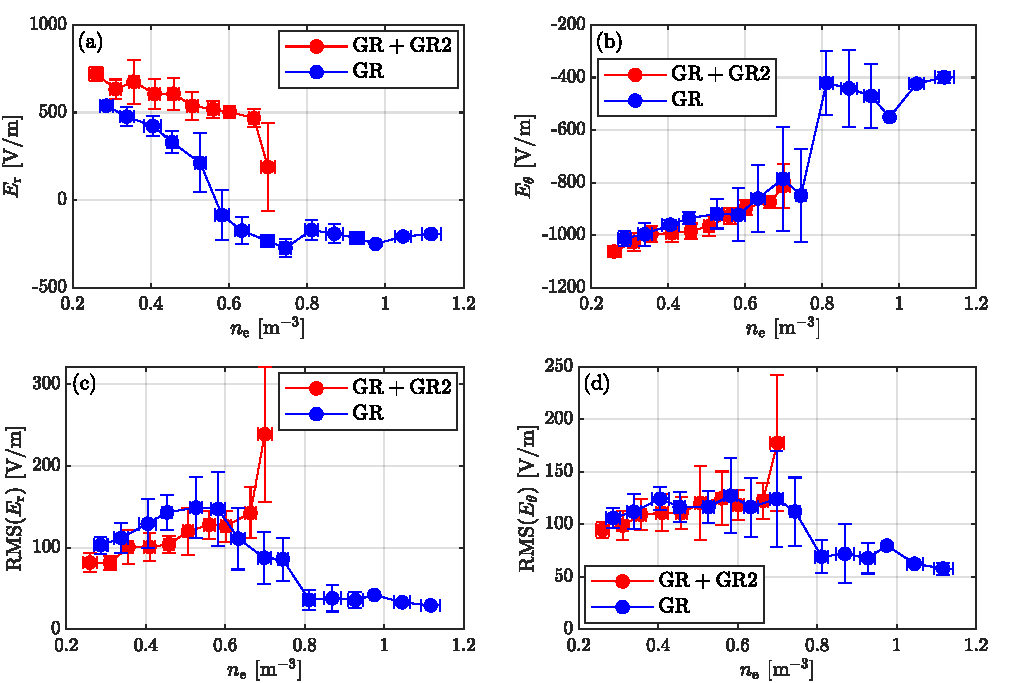
\includegraphics[width=1.0\columnwidth]{Images/transition_1.pdf}
   \caption{Density profiles of (a) radial electric field ($E_{r}$), (b) poloidal electric field ($E_{\theta}$), (c) RMS of the radial electric field 
   ($\mathrm{RMS}(E_{r})$) and (d) RMS of the poloidal electric field ($\mathrm{RMS}(E_{\theta})$). Red and blue lines correspond to ECRH on and off 
   phases, respectively.}
   \label{Fig:transition_1}
\end{figure}

\begin{figure}[!ht]

   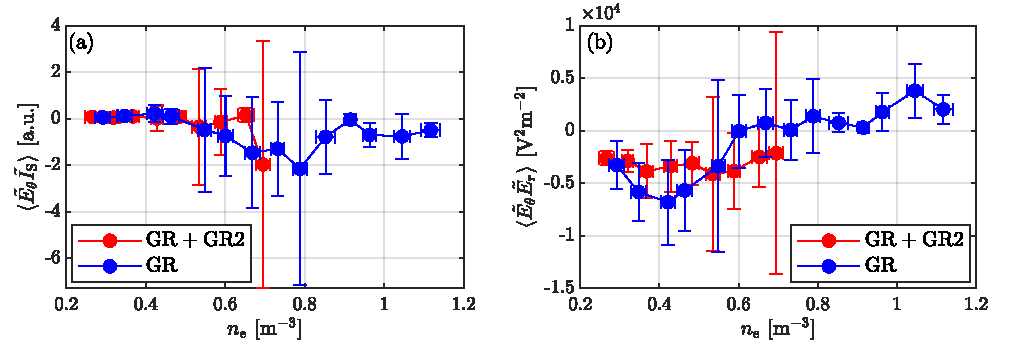
\includegraphics[width=1.0\columnwidth]{Images/transition_2.pdf}
   \caption{Density profiles of (a) Turbulent particle flux ($\langle \tilde{E}_{\theta} \tilde{I}_{S}\rangle$) and (b) Reynolds stress estimated from 
   electric field fluctuations ($\langle \tilde{E}_{\theta} \tilde{E}_{r}\rangle$). Red and blue lines correspond to ECRH on and off phases, respectively.}
   \label{Fig:transition_2}
\end{figure}
\begin{figure}[!ht]

   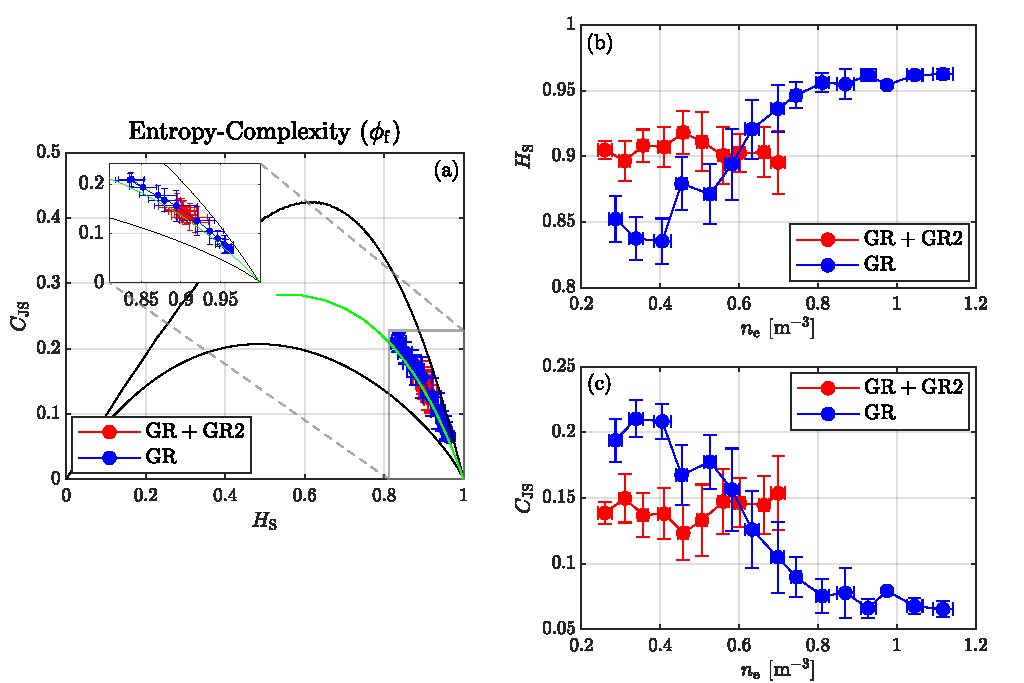
\includegraphics[width=1.0\columnwidth]{Images/transition_3.pdf}
   \caption{(a) Complexity-Entropy causality plane ($C_\mathrm{JS}$-$H_\mathrm{S}$) with $d=5$, for a set of floating potential ($\phi_\mathrm{f}$) signals measured in $\rho=0.8846$,  
   (b) density profiles of the permutation entropy ($H_\mathrm{S}$) and (c) density profiles of the permutation statistical complexity ($C_\mathrm{JS}$).
    Red and blue lines correspond to ECRH on and off phases, respectively.}
   \label{Fig:transition_3}
\end{figure}
\begin{figure}[!ht]

   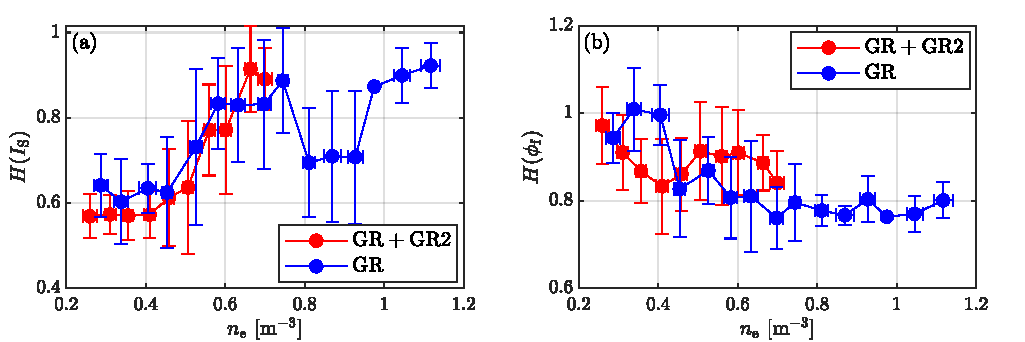
\includegraphics[width=1.0\columnwidth]{Images/transition_4.pdf}
   \caption{Density profiles of (a) Hurst exponent ($H(I_\mathrm{S})$) for a set of ion saturation current ($I_\mathrm{S}$) signals and 
                                (b) Hurst exponent ($H(\phi_\mathrm{f})$) for a set of floating potential ($\phi_\mathrm{f}$) signals.
                                Red and blue lines correspond to ECRH on and off phases, respectively.}
   \label{Fig:transition_4}
\end{figure}
\begin{figure}[!ht]

   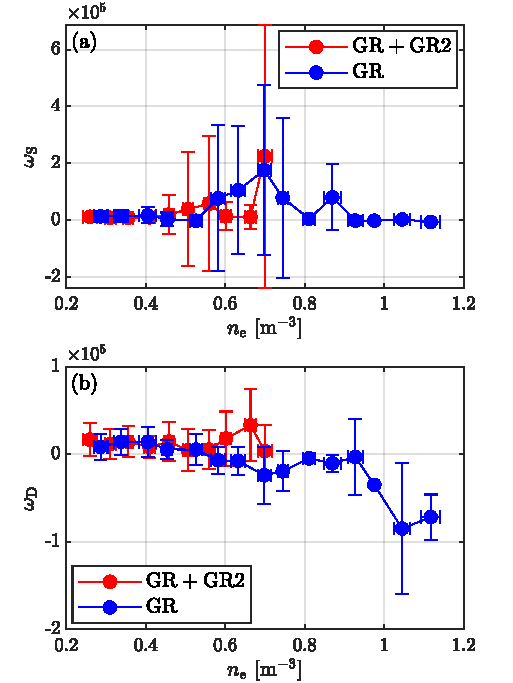
\includegraphics[width=0.5\columnwidth]{Images/transition_5.pdf}
   \caption{Density profiles of (a) rate of turbulence spreading ($\omega_\mathrm{S}$) and 
                                (b) rate of turbulence drive ($\omega_\mathrm{D}$). 
                                Red and blue lines correspond to ECRH on and off phases, respectively.}
   \label{Fig:transition_5}
\end{figure}


\clearpage
\section{Electron Cyclotron emission results}

{\em Note: an example case of ECE $T_e(\rho,t)$ results could be included in the section `Experiments', in order to illustrate the $T_e$ response to modulation, but we don't need an exhaustive study of this, since our goal is turbulence analysis, for which the ECE diagnostic is too limited. So remove most of this.}

~\protect\cite{S_Eguilior_2003}
\begin{equation}
    \frac{3}{2}n_\mathrm{e}\frac{\partial T_\mathrm{e}}{\partial t} + \frac{1}{r}\frac{\partial }{\partial r}(r q_\mathrm{e}) = P^\mathrm{ECRH} - S
    \label{Eq.Transport_1}
\end{equation}

\begin{figure}[!ht]
   \includegraphics[width=1.0\columnwidth]{Images/50019_ECE.pdf}
   \caption{Electron temperature ($T_e$) response to ECRH modulation on axis (shot $50019$). (a) Electron temperature, (b) Root Mean Square of electron temperature in logarithmic scale RMS($T_e$), (c) time derivative of electron temperature ($\partial T_e /\partial t $), (d) variation of time derivative of electron temperature with respect to the radial variation ($\Delta(\partial T_e /\partial t)/\Delta \rho $)}
   \label{Fig:50019_ECE}
\end{figure}

\begin{figure}[!ht]

   \includegraphics[width=1.0\columnwidth]{Images/50024_ECE.pdf}
   \caption{Electron temperature ($T_e$) response to ECRH modulation on axis (shot $50024$). (a) Electron temperature, (b) Root Mean Square of electron temperature in logarithmic scale RMS($T_e$), (c) time derivative of electron temperature ($\partial T_e /\partial t $), (d) variation of time derivative of electron temperature with respect to the radial variation ($\Delta(\partial T_e /\partial t)/\Delta \rho $)}
   \label{Fig:50024_ECE}
\end{figure}

\begin{figure}[!ht]
   \includegraphics[width=1.0\columnwidth]{Images/50031_ECE.pdf}
   \caption{Electron temperature ($T_e$) response to ECRH modulation on axis (shot $50031$). (a) Electron temperature, (b) Root Mean Square of electron temperature in logarithmic scale RMS($T_e$), (c) time derivative of electron temperature ($\partial T_e /\partial t $), (d) variation of time derivative of electron temperature with respect to the radial variation ($\Delta(\partial T_e /\partial t)/\Delta \rho $)}
   \label{Fig:50031_ECE}
\end{figure}

\begin{figure}[!ht]
   \includegraphics[width=1.0\columnwidth]{Images/50033_ECE.pdf}
   \caption{Electron temperature ($T_e$) response to ECRH modulation on axis (shot $50033$). (a) Electron temperature, (b) Root Mean Square of electron temperature in logarithmic scale RMS($T_e$), (c) time derivative of electron temperature ($\partial T_e /\partial t $), (d) variation of time derivative of electron temperature with respect to the radial variation ($\Delta(\partial T_e /\partial t)/\Delta \rho $)}
   \label{Fig:50033_ECE}
\end{figure}

\begin{figure}[!ht]
   \includegraphics[width=1.0\columnwidth]{Images/50035_ECE.pdf}
   \caption{Electron temperature ($T_e$) response to ECRH modulation on axis (shot $50035$). (a) Electron temperature, (b) Root Mean Square of electron temperature in logarithmic scale RMS($T_e$), (c) time derivative of electron temperature ($\partial T_e /\partial t $), (d) variation of time derivative of electron temperature with respect to the radial variation ($\Delta(\partial T_e /\partial t)/\Delta \rho $)}
   \label{Fig:50035_ECE}
\end{figure}

\begin{figure}[!ht]
   \includegraphics[width=1.0\columnwidth]{Images/50036_ECE.pdf}
   \caption{Electron temperature ($T_e$) response to ECRH modulation on axis (shot $50036$). (a) Electron temperature, (b) Root Mean Square of electron temperature in logarithmic scale RMS($T_e$), (c) time derivative of electron temperature ($\partial T_e /\partial t $), (d) variation of time derivative of electron temperature with respect to the radial variation ($\Delta(\partial T_e /\partial t)/\Delta \rho $)}
   \label{Fig:50036_ECE}
\end{figure}


\clearpage


\bibliographystyle{elsarticle-num}
\biboptions{sort&compress}
\bibliography{Bibliography}

\end{document}
